\documentclass[12pt]{book}

% Pachages used for the document: 
\usepackage[top=1in,bottom=1in,left=.75in,right=.75in]{geometry}
\usepackage{titleps}
\usepackage{fancyhdr}
\usepackage{graphicx}
\usepackage{MnSymbol}
\usepackage{pdfpages}
\usepackage{times}
\usepackage[11pt]{moresize}
\usepackage{lipsum} % for dummy texts
\usepackage{ragged2e}
\usepackage{url}
\usepackage[utf8]{inputenc}
\usepackage[T1]{fontenc}
\usepackage[english]{babel}
\usepackage{multirow}
\usepackage{rotating}
\usepackage{hhline}
\usepackage{array}
\usepackage{chngcntr}
\usepackage{parskip}
\usepackage{lettrine}
\usepackage{varwidth}
\usepackage[mathletters]{ucs}
\usepackage{longtable}
\usepackage[table,xcdraw]{xcolor}
\usepackage{minitoc}
\mtcsetdepth{minitoc}{1}
\usepackage{comment}
 \usepackage{appendix}
% configurations for the document :
\renewcommand*{\thesection}{\arabic{section}}
\renewcommand{\arraystretch}{1.5}%cell height scaling
\setlength{\arrayrulewidth}{0.5mm}%table board Thickness
\title{Integrating the Learned Motion  Matching Concept for smart character animation in Unreal engine 5 }
\author{Halloul Tarek}
%\date{}
\graphicspath{./Figures/Images/}
\pagestyle{myheadings}
\pagestyle{fancy}
\fancyhf{}
\setlength{\headheight}{20pt}
\renewcommand{\headrulewidth}{4pt}
\renewcommand{\footrulewidth}{2pt}
\fancyhead[L]{Integrating the LMM Concept for smart character animation in UE5}
\fancyhead[R]{H.T}
%\fancyfoot[L]{}
%\fancyfoot[L]{\textcopyright H.Tarek}
\fancyfoot[R]{\thepage}

%Redefine the titlepage:
\makeatletter
\renewcommand\titlepage{
    \clearpage
    \let\cleardoublepage=\clearpage
    \thispagestyle{empty}
    \if@twocolumn
        \onecolumn
        \@tempswatrue
    \else
        \@tempswafalse
    \fi
    \null\vfil
    \vskip 60\p@
    \begin{center}%
        \setlength{\parskip}{0pt}
        \vskip 3em%
            {\Huge\bfseries\@title \par}%
        \vskip 2em%
        %{\Large\itshape Assisted by lanterns studio\par}%
        \vskip 1.5em%
            {\Large\@date \par}% Add the date, if desired
        \vskip 1.5em%
    \end{center}\par
    \vfil\null
    \if@tempswa
        \twocolumn
    \fi
    \let\cleardoublepage=\clearpage
    \fancyfoot[R]{\thepage}
}
\makeatother

\newenvironment{ConfigureChapter}{
    %\renewcommand{\thechapter}{\Roman{chapter}}
    \centering
        \Centering
        \renewcommand{\thechapter}{\Roman{chapter}}
    }{
    \let\cleardoublepage=\clearpage
    \setcounter{section}{0}
}

% Document content writen here :
\begin{document}
\pagenumbering{Roman}

\includepdf[pages={1,2,3}]{./PFE Repport HalloulTarek.pdf}
\let\cleardoublepage=\clearpage
\dominitoc
\tableofcontents
\listoffigures
\listoftables
\newpage
\paragraph*{\textbf{\huge Abbreviation List:}\\
    \\
    \\
    \\
    MM  : Motion Matching.\\
    LMM : Learned Motion Matching.\cite{LMM}\\
    UE5 : Unreal engine 5.\\
    Mosyp : Motion symphony.\\
    Mocap : motion capture.\\
}
\let\cleardoublepage=\clearpage
\pagenumbering{arabic}
\setcounter{page}{0}

\chapter*{General Introduction}
\addcontentsline{toc}{chapter}{General Introduction}

\lettrine[findent=1pt]{\textbf{M}}{otion} matching technology has revolutionized the field of game development, allowing for more natural and fluid character movements in games. This technology uses machine learning algorithms to match pre-recorded animations to the movements of characters in Real time, creating a more realistic and immersive gaming experience for players. In recent years, motion matching/motion capture has gained widespread adoption in the gaming industry, with major developers such as Epic Games, Ubisoft, and EA Sports incorporating it into their games. One of the most notable examples is EA' FiFa, which uses motion matching/motion capture to create seamless and dynamic character movements in its game world\cite{EA}.\; Ubisoft's Assassin's Creed franchise is another excellent example of the use of motion matching in game development. The franchise has been using motion matching since its 2017 release, Assassin's Creed Origins, to create more realistic and fluid animations for its characters\cite{GDC1}. EA Sports has also adopted motion matching in its sports games, such as FIFA and Madden NFL, to create more realistic player movements and enhance the overall gaming experience\cite{EA1}. Ubisoft's game "For Honor" too had an advancement showcase with this technology providing more details\cite{UBI}. 
Moreover, motion matching has the potential to change the way game developers
approach character animation, allowing for more creative freedom and more dynamic and
engaging game worlds. As motion matching continues to evolve, it is likely to become an even
more integral part of the game development process\cite{GDC2}.
In this report, we will explore the innovations in motion matching technology and its
impact on the gaming industry. We will examine the benefits of motion matching for game
development and discuss the challenges and limitations of this technology. Additionally, we
will analyze case studies of games that have successfully implemented motion matching and
evaluate the potential for future advancements in this field.\\
This report is divided by four chapters, a general context chapter introducing the company and an overview about the project.The second chapter will present more details about the project's system and all the necessary details to its completion.The third chapter will provide the details of the system implementation results. Lastly, a general conclusion and perspective for the system advance improvements.A research annex is provided at the end of the Report to showcase the research results summarized and used to carry on the development process. 
%-------------------------------------------------------------------------------------------------
\begin{ConfigureChapter}
    \chapter{\textbf{General Context}}
    \mtcaddchapter{}
    \minitoc
\end{ConfigureChapter}
\fancyhead[R]{General Context}
\newpage
%-------------------------------------------------------------------------------------------------
\section{Introduction:}
\lettrine[findent=1pt]{\textbf{I}}{n} this chapter, we will provide an overview of the host company and the project we
worked on during the internship. Firstly, we will introduce the company and describe the
general environment in which it operates. Next, we will outline the project's objectives and
goals, followed by a discussion of the primary issue that the project aimed to address.
Additionally, we will detail the methodology used to tackle the problem and highlight our
approach to managing the project's progress and development. Overall, this chapter will provide a comprehensive understanding of the project and the strategies employed to achieve its goals.
\section{Hosting Company:}
Lanterns Studio is a Tunisian gaming company that was established in 2019 and is
headquartered in Tunis. The company specializes in delivering advanced technology solutions
that help accelerate its clients' digital transformation, as well as providing extended reality
applications and motion capture services. With a team of highly skilled and knowledgeable
employees and strategic partnerships with industry leaders, Lanterns Studio is dedicated to
delivering cutting-edge solutions that meet the evolving needs of its clients.
It is composed by a highly skilled team of various domains related to IT , CG , branding and media content: from mobile apps development to AR/VR experiences, PC to
console video games \cite{url-1}.
\begin{figure}[!h]
    \centering
    
\includegraphics[width=8cm]{./Figures/Images/Lanternslogo.png}\\
    \caption{Lanterns studio}
    \label{Lanterns studio}
\end{figure}
Lanterns Studio provides a range of innovative solutions across diverse industries,
including information technology, computer graphics, branding, and media content. The
company offers a comprehensive suite of services, from mobile application development to
augmented and virtual reality experiences, and from PC to console video games. With a focus
on creativity and technology, Lanterns Studio is committed to providing its clients with
solutions that are tailored to their unique needs and goals, and that push the boundaries of what's possible in the digital landscape.
\begin{center}
    \begin{varwidth}{\textwidth}
        Company:        Lanterns\\
        Creation Date:  2019\\
        Category:       Company\\
        Sector:         Gaming\\
        Address:        Rue de l'energy, Tunis\\
        City:           Tunis\\
        Zip Code:       2035\\
        Country:        Tunisia\\
        Phone:          +216 23586707\\
        Website:        https://lanterns-studios.com/\\
        E-mail:         info@lanterns-studios.com\\
    \end{varwidth}
\end{center}

\section{Company mission}
In order to stay the market leader, Lanterns Studios is keeping its teams up to date with the
latest technologies and media trends who are keen to prove themselves in this industry and
invest in training new profiles and talents within the company.

\section{Project overview:}
The objective of this project is to develop a motion matching system, a technology extensively utilized in game development to achieve
realistic and coordinated movements for individual characters or entities. The system involves the creation of "agents",
which represent the characters or entities within the game. Each agent is equipped with specific rules and behaviors,
such as moving toward designated destinations or navigating around obstacles. To enhance the animations further, motion matching
comes into play. This technique involves capturing a diverse range of motion data and then utilizing an algorithm to match the desired
movement to the most suitable motion clip. The result is a more natural and fluid animation that is responsive to the game's environment
and other agents within the scene. By combining these two technologies, developers can create expansive, dynamic crowds capable of realistic
and reactive movements within the game's environment and events. Motion matching systems find particular value in games that demand lifelike
and dynamic crowds, such as sports games or open-world games featuring large cities or events.

\section{Problem Description}
The need for larger, more immersive and dynamic worlds in interactive applications, such as
video games, has presented a challenge for creating characters that can respond realistically and
naturally in an increasing number of different situations. This is exacerbated by the growing
demand for high-quality animations, which requires a significant amount of data. AAA video
games, in particular, can contain tens of thousands of unique animations that must be triggered
in the correct context, making the task of producing responsive and natural characters even
more difficult. [Holden 2018] \cite{url-2}.
Clavet and Büttner [2015] proposed Motion Matching as a technique for searching a vast
database of animations to find the one that best matches a given context \cite{url-3}.
Despite its effectiveness , Motion Matching’s memory usage can become a major issue when
dealing with large amounts of animation data. As the amount of data used increases, so does
the memory required to store and access that data, resulting in a linear increase in memory
usage. This presents a challenging trade-off for developers and animators, as increasing the
amount of data used can lead to more expressive and complex animations, but it also requires
more memory and computational resources.
The creation of a perfect animation system for NPCs where the solution provides with as
much detailed movements as possible as well as visually attractive was truly difficult to
maintain and provide. It is difficult to create such system with \textbf{state machines}alone, it implicates adding multiple animation record and using too much \textbf{blend trees} at the same time with a single character animation (Which uses an amount of memory and calculations needed to achieve an acceptable result which is incredibly large) and results with non-organized projects and sometimes messy animation structures, that’s what traditional animation technique is handling.
\begin{figure}[!h]
    \centering
    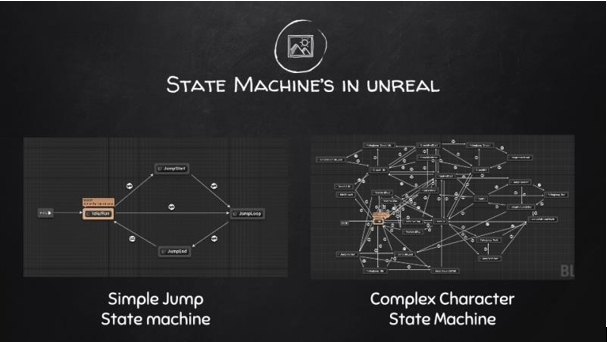
\includegraphics[scale=0.8]{./Figures/Images/complexeStateMachines.png}
    \caption{Complex state machines}
    \label{Complex state machines}
\end{figure}
\begin{figure}[!h]
    \centering
    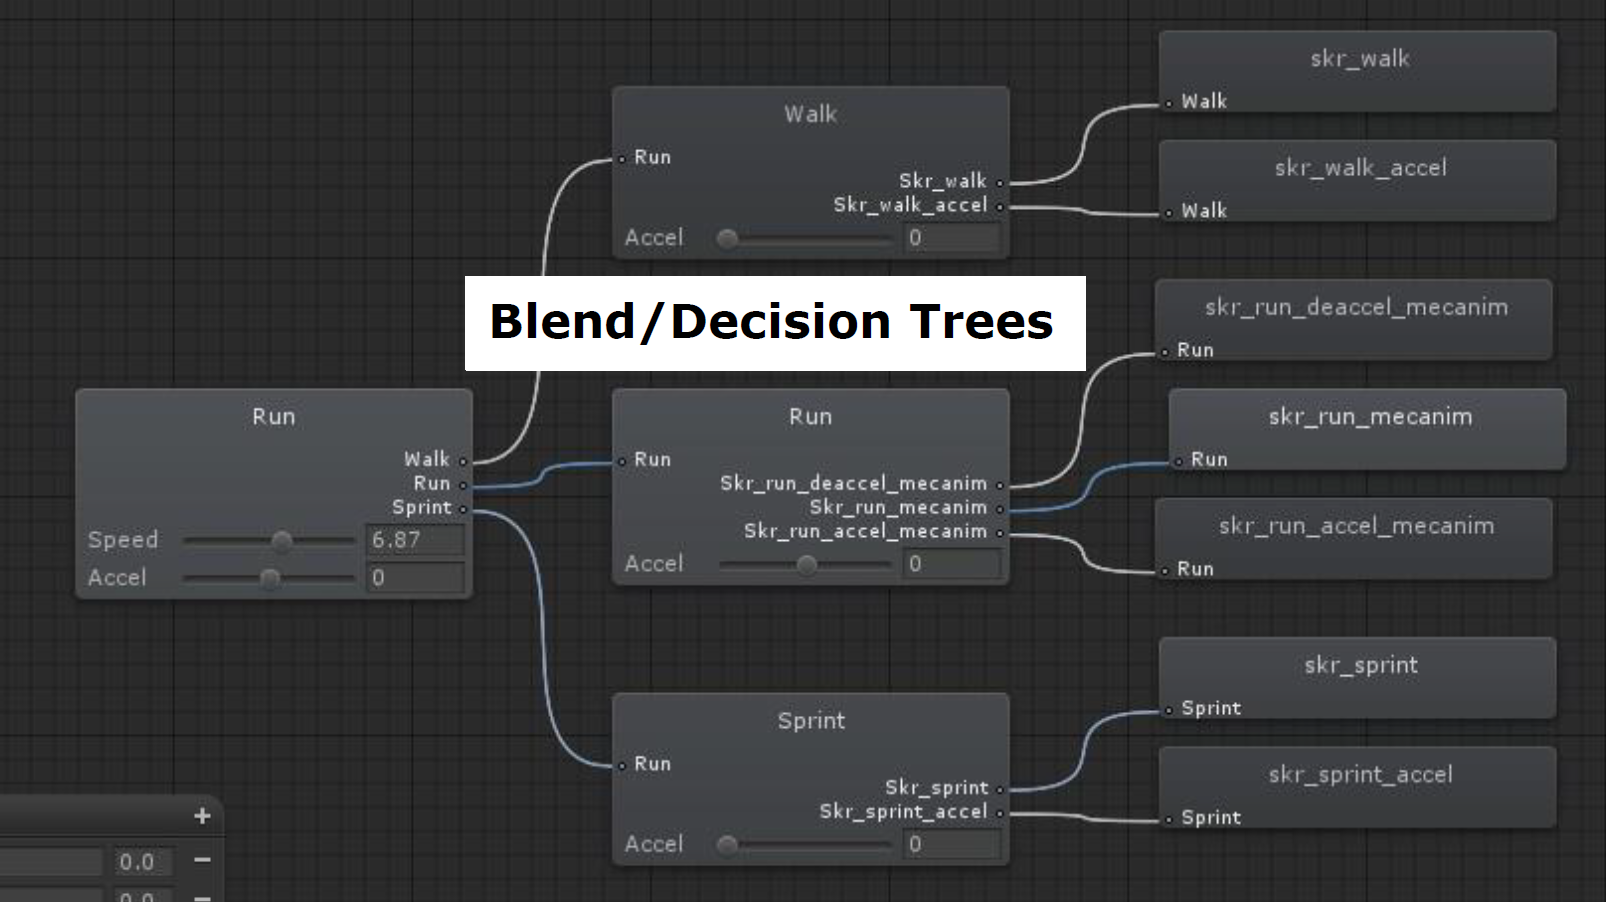
\includegraphics[scale=0.3]{./Figures/Images/blendtrees.png}
    \caption{Complex Blend trees}
    \label{Complex Blend trees}
\end{figure}
To create a cutting-edge animation system for our game, we conducted an extensive study of existing
technologies and techniques in the field. This involved analyzing various crowd simulation
and motion capture methods used in popular games, identifying their strengths and limitations.
Additionally, we thoroughly reviewed academic literature and research papers to gain a deeper
understanding of the underlying principles and algorithms related to animation. Through this
comprehensive study, we were able to identify the most effective techniques and technologies to
ensure the development of a realistic and dynamic animation system. \textbf{Motion matching},
a revolutionary technology in game development, addresses the challenges associated with
traditional animation techniques. It overcomes the time-consuming and costly process of creating
numerous unique animations for different scenarios by seamlessly blending motion data using a
database and algorithms. This results in smooth, natural, and responsive movements that adapt to
the game's environment and events in real-time.
\newpage
\section{Study of the existing:}
In the past, creating realistic crowd systems in games was a difficult task that required
significant development resources. Before the advent of motion matching, game developers
typically used pre-animated crowd animations or simple rule-based systems to simulate crowds.
These approaches were limited in their ability to create truly dynamic and realistic crowds, as
the animations were often repetitive and lacked responsiveness to the game's environment and
events. Rule-based systems were also limited in their ability to create natural movement, as they
relied on simple rules that did not account for complex behaviors or interactions. As a result,
developers often had to resort to various tricks and techniques, such as duplicating models and
animations or reducing the number of characters in a crowd, to achieve the desired effect.
However, these solutions were often unsatisfactory, and the resulting crowds were often static
and lacked the realism and dynamism that modern games require.

\subsection{Case of study:}
To undertake this ambitious project successfully, it is crucial to comprehend its specific
requirements and intricacies. Thus, following the establishment of the project's overarching
context, this section is dedicated to examining comparable endeavors that share similar visions or to be more precise, search and test similar products implementing the same mechanics.

\subsubsection{\underline{* Virtual Motion Matching V3:}}
Virtual Motion Matching V3 represents the cutting-edge evolution of motion matching
technology in game development. This advanced system employs a sophisticated algorithm
to seamlessly match a wide array of motion data, enabling characters and entities to move
with unparalleled realism and fluidity. With V3, developers can create lifelike animations
that dynamically respond to the game's environment and interactions. This groundbreaking
technology sets new standards for immersive gameplay, enhancing the player's experience
in virtual worlds like never before.
\begin{figure}[!h]
    \centering
    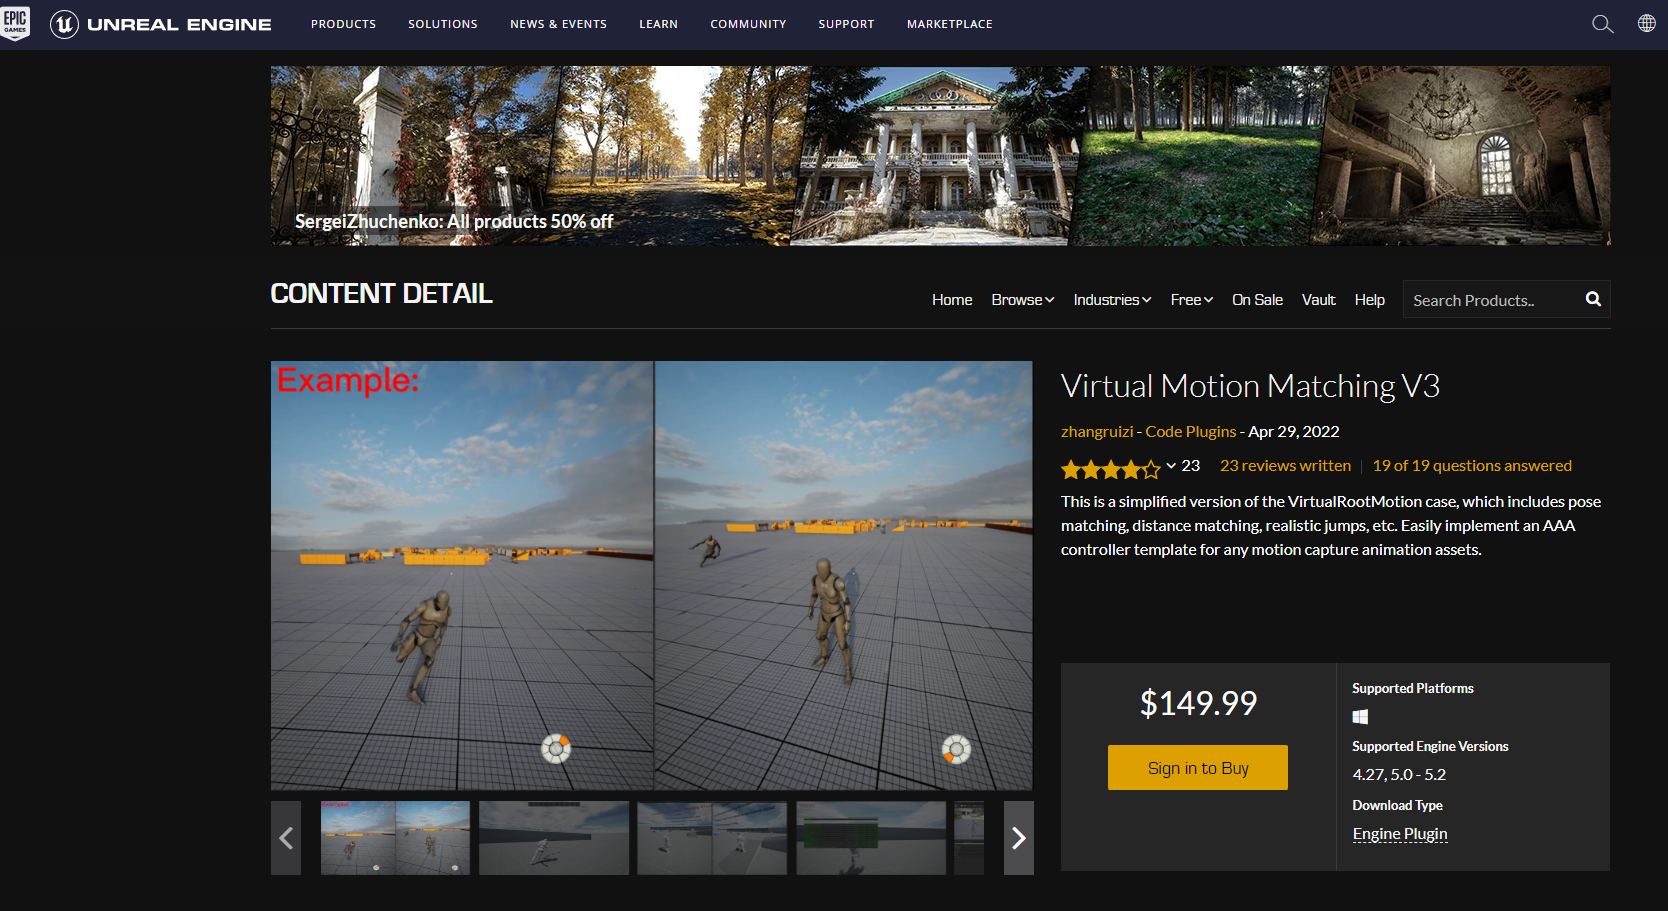
\includegraphics[scale=0.3]{./Figures/Images/virtual-motion-matching.png}
    \caption{Virtual Motion Matching V3}
    \label{Virtual Motion Matching V3}
\end{figure}
The Virtual Motion Matching V3 plugin offers streamlined animation workflows but may not encompass the extensive feature set of Motion Symphony. While it provides efficient solutions, some advanced functionalities present in Motion Symphony might be absent, catering to different user needs and priorities.

\subsubsection{\underline{* Motion Matching System Plugin}} 
Motion Matching System allow to create realistic, grounded animation system for character and NPC's using Motion Matching developed by Filmstorm.\cite{url-5} 
%https://www.unrealengine.com/marketplace/en-US/product/motion-matching-system
\begin{figure}[!h]
    \centering
    \fbox{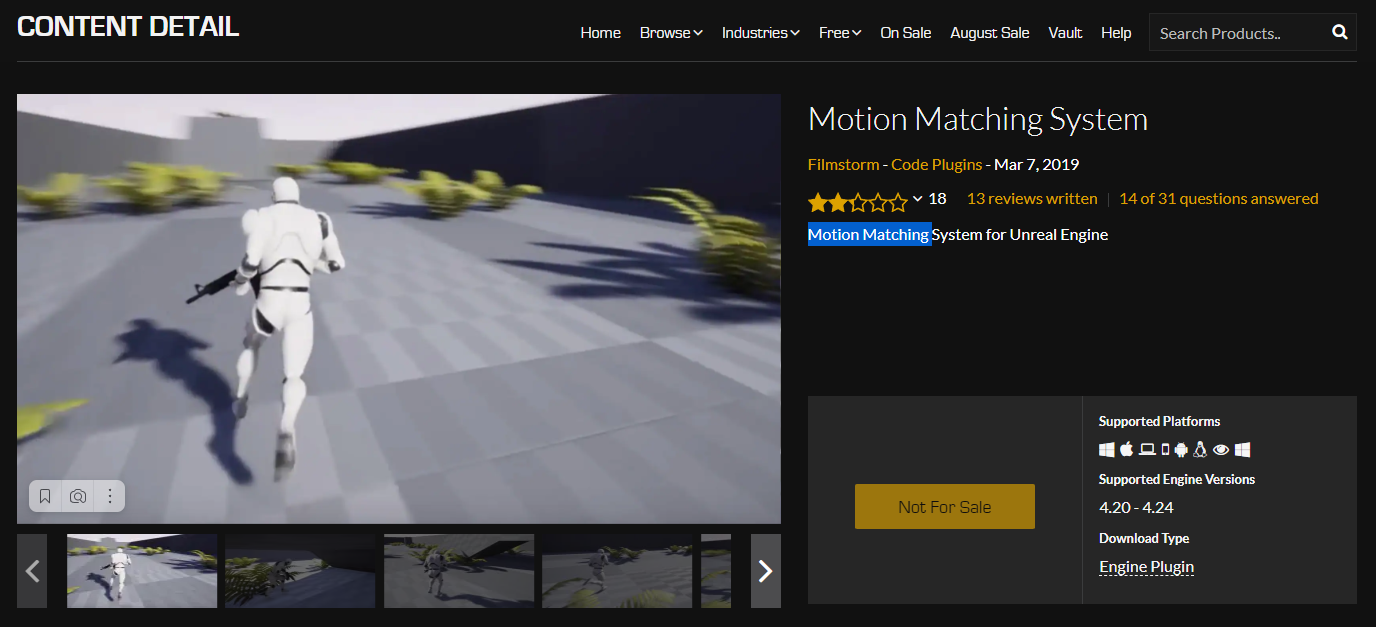
\includegraphics[scale=0.3]{./Figures/Images/MotionMatchingPlugin.jpg}}
    \caption{Motion System in Epic's Marketplace.}
   \end{figure}

Below we will mention the main features offered by this plugin :

\begin{list}{-}{}
  \item Motion Matching
    \item Designed for optimal performance in game
     \item  Pre-packed with animations to test the motion matching system
\end{list}

\subsubsection{\underline{* Motion symphony:}}
Motion Symphony is an animation plugin, a suite of cutting edge animation tools that enable
high fidelity character animation while also simplifying animation graph. It was designed in a modular way to help improve flexibility and re-usability of
data, Creating these modules in the right order is important.
\begin{figure}[!h]
    \centering
    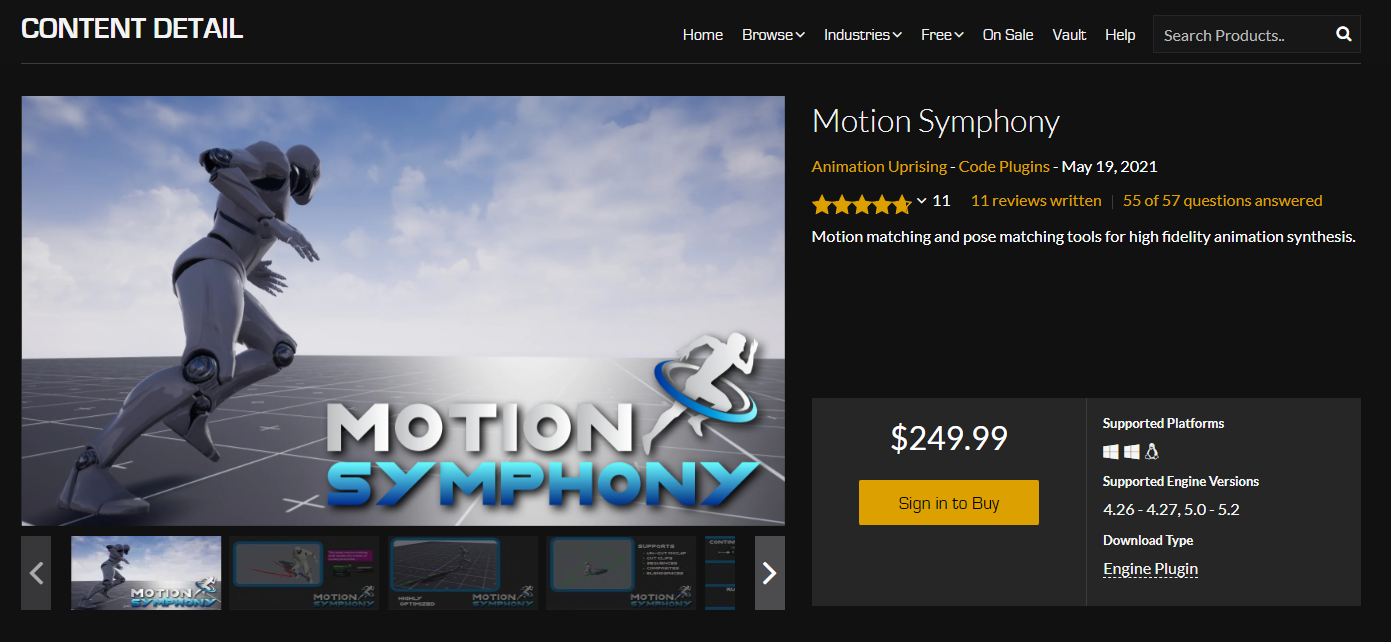
\includegraphics[scale=0.3]{./Figures/Images/Motion Symphony/MotionSymphony.jpg}
    \caption{Motion Symphony in Epic’s Marketplace}
    \label{Motion Symphony in Epic’s Marketplace}
\end{figure}
The Motion Symphony plugin offers remarkable capabilities, enhancing animation workflows effectively. However, its resource-intensive nature, demanding significant memory usage, might pose challenges for projects with limited resources. Additionally, it's important to note that Motion Symphony is a premium product, requiring a financial investment for access to its advanced features.

\subsubsection{\underline{* Summary tables}}
The Table down bellow presents the difference between both plugins in unreal engine and shows the characteristics and the criticisms of each one. This table provide us with a summary of the systems major disadvantages to take into consideration when developing a best solution to solve each one's shortcomings.
We'll be selecting a technology between both as a base plugin to test out and see its the best behaviour. And that, to later on, include it into our solution with a major correction in its shortcomings.
\begin{figure}[!h]
    \centering
    
\includegraphics[scale=0.5]{./Figures/question.png}
\end{figure}
\newpage
% Please add the following required packages to your document preamble:
% \usepackage[table,xcdraw]{xcolor}
% If you use beamer only pass "xcolor=table" option, i.e. \documentclass[xcolor=table]{beamer}
% \usepackage{longtable}
% Note: It may be necessary to compile the document several times to get a multi-page table to line up properly
\begin{longtable}[c]{|l|l|l|}
\caption{Summary table}
\label{ Existing projects capabilities and criticism}\\
\hline
\multicolumn{1}{|c|}{\textbf{Plugin}} & \multicolumn{1}{c|}{\textbf{Characteristics}} & \multicolumn{1}{c|}{\textbf{Criticism}} \\ \hline
\endfirsthead
%
\multicolumn{3}{c}%
{{\bfseries Table \thetable\ continued from previous page}} \\
\hline
\multicolumn{1}{|c|}{\textbf{Plugin}} & \multicolumn{1}{c|}{\textbf{Characteristics}} & \multicolumn{1}{c|}{\textbf{Criticism}} \\ \hline
\endhead
% 
Motion Symphony & \begin{tabular}[c]{@{}l@{}}Compatible with a wide\\ range of platforms and \\ endorsed by Unreal Engine\\ versions 4.20 to 4.24, this\\ plugin is available for free\\ on Epic's marketplace and\\ comes integrated with a \\ set of MoCap animations.\end{tabular} & \begin{tabular}[c]{@{}l@{}}Lack of clear guidance on \\ utilizing the plugin, coupled\\ with dissatisfaction evident\\ in many reviews, and the \\ plugin's compatibility with\\ engine versions falling below\\ our company's standards.\end{tabular} \\ \hline

\begin{tabular}[c]{@{}l@{}}Motion Matching \\ System\end{tabular} & \begin{tabular}[c]{@{}l@{}}Compatible with both \\ Windows and Linux \\ operating systems, this \\ plugin is endorsed by \\ Unreal Engine versions \\ 4.26 to 4.27, as well as \\ 5.0 to 5.2. It boasts an \\ extensive range of features, \\ encompassing even \\ experimental options. \\ The plugin is thoroughly \\ documented and has received \\ excellent reviews on the \\ marketplace.\end{tabular} & \begin{tabular}[c]{@{}l@{}}Expensive and scalability\\ problem.\end{tabular} \\ \hline
\end{longtable}

After reviewing the comparison table, we've opted to proceed with Motion Symphony as an actual demonstration of motion matching. This selection will allow us to push its boundaries and evaluate its potential by creating a prototype.

\subsection{Suggested Solution:}
Learned Motion Matching (\textbf{provided in the annex section \ref{appendix:LMM}}) is an animation technique that leverages machine learning to improve the performance and scalability of Motion Matching-based animation systems and is, till now, the ideal solution for AAA games. We will implement this solution after more research and inspections for its production probabilities.
 \begin{figure}[!h]
    \centering
    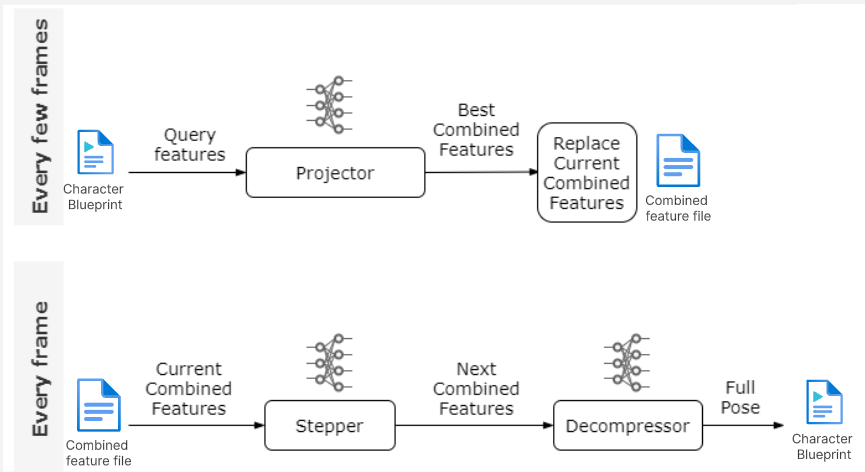
\includegraphics[scale=0.7]{./Figures/finalLMM.PNG}
    \caption{LMM final functional structure}
    \label{LMM final functional structure}
\end{figure}

\section{State of Animation in Game Development}
In this section, we sill provide a brief and abbreviated explanations about the technical animation concepts used in the game development as the MM and LMM's system.

\subsection{Animation system in game Development}
\lettrine[findent=1pt]{\textbf{I}}{n} gameplay programming, gameplay animation is generally considered the most important and attractive part of the whole product. It is a combination of different elements like Animation Clips, which encapsulate specific motion sequences for characters and objects. These clips are governed by the Skeletal Rig, a structure defining how character parts move in response to animations. To ensure fluid transitions between animations, State Machines come into play, managing the character's behavioral states, such as walking, running, or jumping. Blending techniques further enhance realism by smoothly combining various animations, allowing for seamless and dynamic character movements in gameplay experiences.
You can find more details about its concept in the annex section \ref{appendix:state}.

\subsection{Motion Matching Concept}
\lettrine[findent=1pt]{\textbf{I}}{n} this subsection, we will provide a brief explanation about what is a motion matching system throw the research results of the annex's section \ref{appendix:MM}.\\
The Motion Matching pipeline system works as the follows:
\begin{itemize}
    \item Mocap is tweaked, imported and marked up.
    \item At runtime, the animation system makes a request (Desired trajectory and event constraints)
    \item The animation system continuously finds the best Peace of data to play.
    \item The animation system modify the result found to precisely match the gameplay and the environment which the character is in.
\end{itemize}
The Motion Matching system operates in a sequential process to generate lifelike character animations. First, it analyzes the input from player controls and game context. Next, it queries the motion database to retrieve relevant animation clips. The selected clips are blended together seamlessly to create a smooth transition. Finally, the resulting animation is applied to the character's skeletal rig, yielding natural and responsive in-game movements with procedural warping.
\begin{figure}[!h]
    \centering
    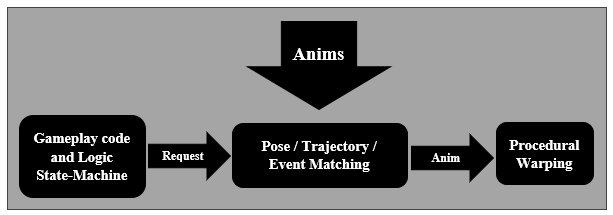
\includegraphics[scale=1.1]{./Figures/Images/motion matching process diagram.PNG}
    \caption{Motion Matching Pipeline in a simple Diagram}
    \label{Motion Matching Pipeline in a simple Diagram}
\end{figure}

\section{Project Methodology:}
\begin{comment}
In order to ensure the reliability of software, it is crucial to establish a well-defined work
methodology and a comprehensive monitoring process prior to initiating a computer project.
This approach outlines a systematic procedure aimed at formalizing the early stages of system
development, with the goal of enhancing the alignment between the development process and
the specific requirements of the client.
\subsection{Scrum presentation:}
Agile Scrum is an iterative and incremental project management framework that promotes
flexibility, collaboration, and continuous improvement in software development. It emerged as
a response to the challenges faced by traditional project management approaches, which often
struggled to adapt to rapidly changing requirements and lacked effective communication and
transparency. At its core, Agile Scrum follows the principles of the Agile Manifesto,
emphasizing individuals and interactions, working software, customer collaboration, and
responding to change. It embraces an iterative and time-boxed approach, dividing the project
into small, manageable units called sprints. Each sprint typically lasts two to four weeks and
focuses on delivering a tangible and potentially shippable product increment.
The Scrum framework consists of three primary roles: the Product Owner, the Scrum Master,
and the Development Team.
\subsection{Development Methodology:}
To achieve the project's objectives efficiently while ensuring high-quality software, selecting the most suitable development approach
is a pivotal decision in the project's life cycle. Following a thorough assessment of various factors, we have structured the project into
multiple iterations, each concentrating on distinct components. At the completion of each iteration, a tangible increment will be delivered.
Consequently, we have chosen to adopt the Agile SCRUM development process to effectively accomplish these iterative goals.
\begin{figure}[!h]
    \centering
    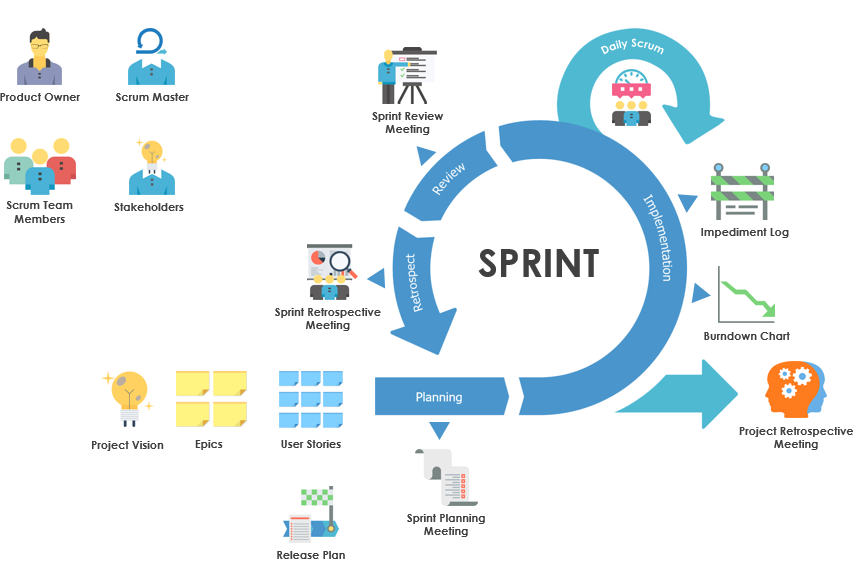
\includegraphics[scale=0.6]{./Figures/Images/the-agile-scrum-framework-1.png}
    \caption{Scrum Life Cycle}
    \label{Scrum Life Cycle}
\end{figure}
\newpage
%\subsubsection{Agile methodology:}

% The Product Owner represents the stakeholders and ensures that the product backlog, a 
% prioritized list of features and requirements, is well-defined and reflects the customer's needs. 
% The Scrum Master facilitates the Scrum process, removes any impediments that hinder the 
% team's progress, and fosters a productive and collaborative environment. The Development 
% Team, consisting of cross-functional members, is responsible for delivering the product 
% increment at the end of each sprint. Key practices within Agile Scrum include daily stand-up 
% meetings, where team members share progress, discuss challenges, and plan the day's work; 
% sprint planning, where the team selects the backlog items to be worked on in the upcoming 
% sprint; and sprint review and retrospective, where the team demonstrates the completed work 
% to stakeholders and reflects on the sprint to identify areas for improvement. 
% One of the significant benefits of Agile Scrum is its emphasis on customer collaboration 
% and early and frequent delivery of working software. This iterative approach allows for 
% continuous feedback, enabling the team to adapt and adjust based on customer needs and
% changing requirements. Additionally, the transparency and regular communication within 
% Scrum foster a shared understanding and alignment among team members and stakeholders.
% \subsection{Scrum Roles:}
% SCRUM encompasses three primary roles, which will be detailed in the table presented 
% subsequently: 
% \begin{itemize}
%     \item \underline{Product Owner:}\\
%     The Product Owner serves as the designated representative of the client within a Scrum 
%     project. They act as the primary point of contact for the Scrum Master and team members, 
%     assuming responsibility for articulating the product's requirements and crafting the 
%     specifications. Collaborating with functional experts, the Product Owner may receive assistance 
%     in defining the specifications. Additionally, they play a crucial role in establishing and 
%     prioritizing user stories for each sprint.\\ 
%     \item \underline{Scrum Master:}\\
%     He fulfills the role of overseeing the method's execution and ensuring its objectives are 
%     met. While not assuming the position of a Project Leader, he assumes the responsibility of 
%     eliminating any potential hurdles that could impede the team's progress and hinder the project's 
%     advancement throughout the multiple sprints.\\ 
%     \item \underline{Development Team:}\\
%     These individuals are responsible for attaining the sprint goals and delivering a functional 
%     product by the end of the iteration. They encompass a range of roles, including developers, 
%     architects, and functional testers. The team maintains direct communication with the client.\\
% \end{itemize}
% \subsection{Benefits Offered by Agile:}
% Agile emphasizes four primary values, including the prioritization of people and interactions over 
% processes and tools, valuing functional software over extensive documentation, placing greater 
% importance on customer collaboration than contractual agreements, and embracing adaptability 
% and responsiveness to change instead of rigidly adhering to a predetermined plan.
% \subsection{Fundamental aspects of Agile Method development principles:}
% A collective of software developers reached a consensus to formulate an agile manifesto that emphasizes responsiveness to change and contrasts with the principles favored in the Waterfall approach. Their stated principles are as follows:
% \begin{itemize}
%     \item Prioritize continuous customer satisfaction by delivering valuable software.
%     \item Embrace changes at any stage of the project, irrespective of its commencement or conclusion.
%     \item Aim for frequent delivery of fully operational software within short intervals, typically spanning weeks rather than months.
%     \item Foster ongoing collaboration between clients and the project team.
%     \item Emphasize the significance of face-to-face communication among all involved parties.
%     \item Establish projects around motivated individuals within a supportive environment.
%     \item Consider functional software as the primary measure of progress.
%     \item Foster a sustainable pace for long-term development.
%     \item Maintain a consistent focus on technical excellence and sound design practices.
%     \item Recognize simplicity as a crucial element of effective agile management.
% \end{itemize}
% \subsection{The Advantages of Agile Development Methods:}
% Amidst the age of digital transformation, as numerous organizations transition towards digital 
% workplaces, the Agile methodology seamlessly aligns with companies aiming to revolutionize project 
% management and overall operational practices:
% \begin{itemize}
%     \item Enhanced flexibility and adaptability.
%     \item Improved efficiency and productivity.
%     \item Heightened transparency and visibility.
%     \item Deliverance of superior quality products.
%     \item Reduced likelihood of missing goals.
%     \item Increased stakeholder engagement and satisfaction.
% \end{itemize}    
\end{comment}
In our project, we will use the V Development Methodology, a structured approach to software development. This method employs a sequential process resembling a V shape, with development on the left side and testing on the right. It begins with comprehensive requirement analysis, followed by system architecture, coding, and component design. Corresponding testing phases run in parallel, including unit, integration, system, and user acceptance testing. The strength of this model lies in its clear correlation between development activities and testing outcomes, facilitating early issue detection. However, its sequential nature can be less adaptable to changing requirements. Popular in safety-critical and regulated sectors, the V-Model ensures rigorous testing and validation, making it a preferred choice in such domains.
\begin{figure}[!h]
    \centering
    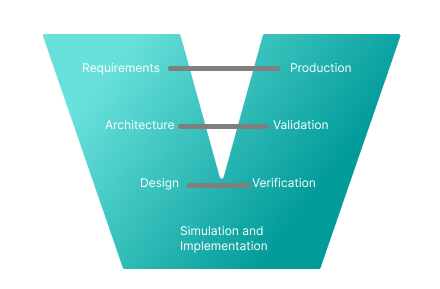
\includegraphics[scale=0.9]{./Figures/V Dev.png}
    \caption{The V Methodology in Game Development}
    \label{The V Methodology in Game Development}
\end{figure}\\

\subsection{Gantt Diagram:}
The diagram (figure 1.10) bellow shows the project partition and the cycle of work, research and development confronted in the internship.
\begin{sidewaysfigure}
    \centering
    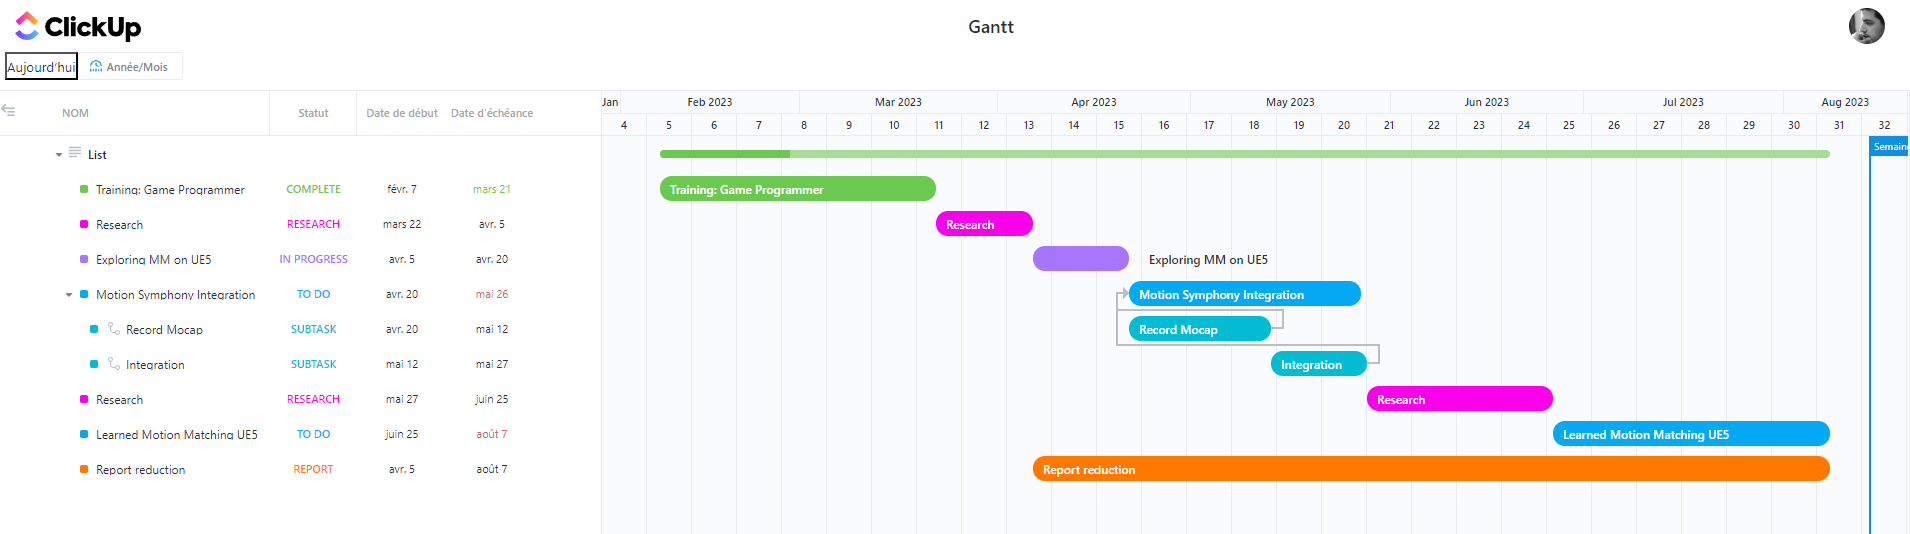
\includegraphics[scale=0.4]{./Figures/Images/gantt.png}
    \caption{Gantt Diagram}
    \label{Gantt Diagram}
\end{sidewaysfigure}

\subsection{Conclusion:}
In this chapter we presented the details about the company as the projects problematic and its primary objective, which is the creation of a motion matching system that can simulate the most natural animations as realistic as possible. And so, without using animation Blueprints or a state machines based system.    

\begin{comment}
\begin{ConfigureChapter}
    \fancyhead[R]{Needs analysis and specification}
    \chapter{\textbf{Needs analysis and specification}}
    \minitoc
\end{ConfigureChapter}

\section{Introduction:}
\lettrine[findent=1pt]{\textbf{T}}{his} chapter presents the different actors of the application and a detailed
description of the different functional and non-functional needs and ends with the planning of sprints and users
stories as a product backlog.
\end{comment}
%-------------------------------------------------------------------------------------------------------
\begin{ConfigureChapter}
    \chapter{\textbf{The Learned motion matching system}}
    \minitoc
\end{ConfigureChapter}
\fancyhead[R]{The LMM system}
%-------------------------------------------------------------------------------------------------------
\newpage
\section{Introduction:}
\lettrine[findent=1pt]{\textbf{T}}{his} chapter introduces the LMM technology along with its essential foundations required for its proper implementation. We also offer comprehensive explanations to ensure a thorough comprehension of its concept. Additionally, we outline the participants involved in its application, furnish a detailed account of both functional and non-functional requirements, and conclude by presenting the development plan structured as a series of sprints, accompanied by a user story-based product backlog.

\section{Project Objective:}
Our project endeavors, for making professional and more advanced games that are able to:\\
• Implement the Motion Matching system solution in a player or NPC
character.\\
• Test the Player or the NPC both the motion matching
technologies.\\

\section{Requirements definition}
\subsection{Functional and nonfunctional needs:}
\lettrine[findent=1pt]{\textbf{I}}{n} this section, we'll be showing the structure of the project throw the UML conceptual study language.We will present in a precise and simple way the LMM system.

\begin{comment}
    \subsubsection{\underline{Motion Symphony's and the LMM's Functional needs:}}
The MS system's functional requirements encompass its core functionality, which primarily
originates from the game developer. The objective of this system is to enable him to:
\begin{itemize}
    \item Create Motion Configuration Asset in the Unreal 5 project.
    \item Create the Motion Calibration Asset in the Unreal 5 project.
    \item Create the Motion Data Asset in the Unreal 5 project. within it, the game developer must configure its motion Data asset,add animations to the file and configure them,
          preprocess its information and lastly has the choice to tag them if needed.
    \item Add Trajectory Generator Component in the Unreal 5 project.
\end{itemize}
As for the LMM system, its core functional requirements are listed as follows bellow:
\begin{itemize}
    \item Update the motion Database of animations in the Unreal 5 project.
    \item configure Motion Matching in the Unreal 5 project.
    \item Load the Motion Data in the Unreal 5 project.
    \item Add any animation into any motion dataset or existing ones.
\end{itemize}
The game player is able here to:
\begin{itemize}
    \item Perform Motion Matching while playing the game that uses the LMM system.
\end{itemize}
\begin{figure}[!h]
    \centering
    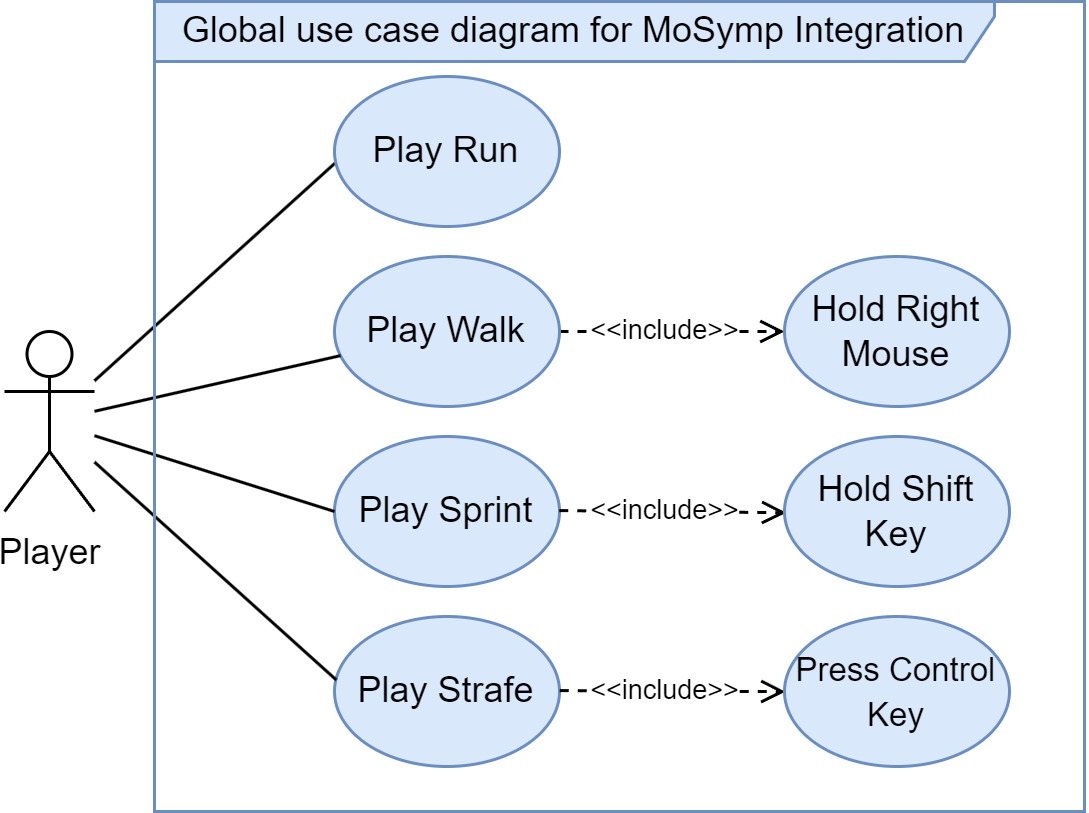
\includegraphics[scale=0.2]{./Figures/uml/UserCaseMoSymp.png}
    \caption{Motion Symphony General Use case Diagram}
    \label{Motion Symphony General Use case Diagram}
\end{figure}
\begin{figure}[!h]
    \centering
    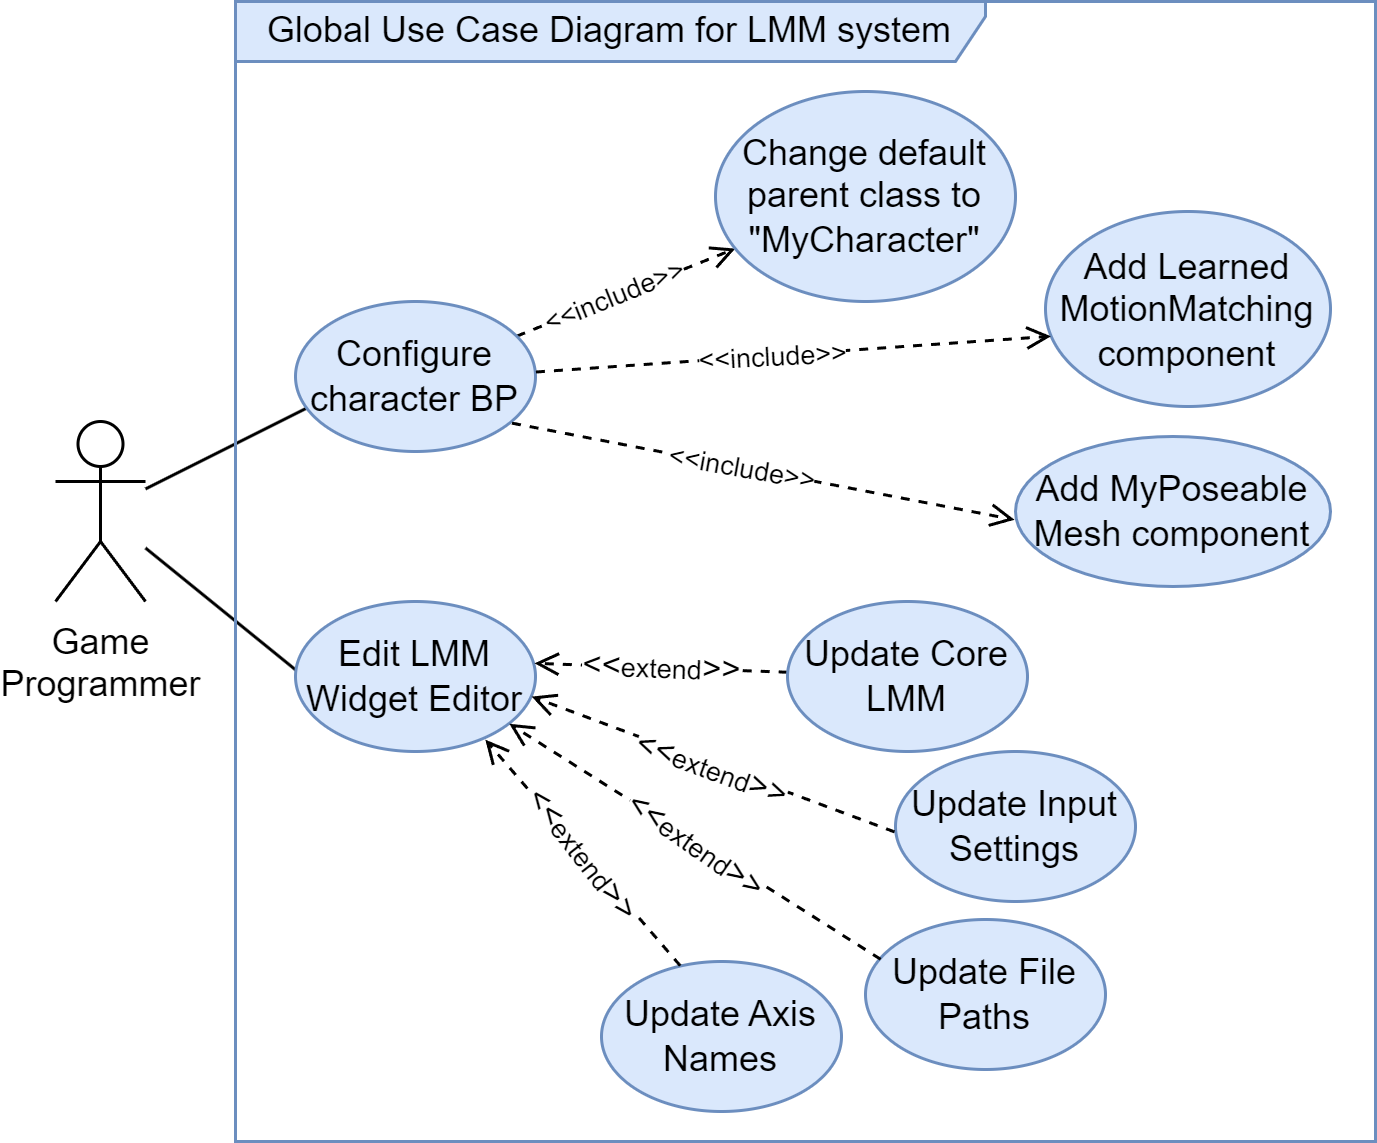
\includegraphics[scale=0.2]{./Figures/uml/LMMUseCaseGlobal.png}
    \caption{LMM General Use case Diagram}
    \label{LMM General Use case Diagram}
\end{figure}

\newpage

\subsection{Nonfunctional needs:}
In addition to the fundamental prerequisites, the project must also fulfill specific criteria
related to performance and design specifications, encompassing:
\begin{itemize}
    \item \underline{Performance:}
          The foremost requirement for the system is its efficiency, which entails meeting all user
          requirements optimally through its functionalities.
    \item \underline{Maintainability:}
          As an integral component of this project, it is imperative that the system possesses the
          quality of extensibility.
    \item \underline{Understandability:}
          \begin{itemize}
              \item Design, architecture, and code that are straightforward and accessible for
                    comprehension and learning.
              \item The capacity for other developers and animators to implement changes swiftly
                    and efficiently.
              \item Supporting the unreal project versions from unreal engine 5 to 5.1
          \end{itemize}
    \item \underline{Efficiency:}
          \begin{itemize}
              \item Satisfactory promptness in addressing user interactions.
              \item Error Recovery:
                    The duration required to restore or redo work following an error.
              \item Supporting the unreal project versions from unreal engine 4 to 5.
          \end{itemize}
\end{itemize}
\section{Needs analysis}
\end{comment}

The process of defining requirements involves identifying and explaining the features offered by the solution itself. In this section, we focus on Needs analysis. We start by identifying every system's actors, then list their functional and non-functional requirements.

\subsection{Actor Identification}
Within the motion symphony and the LMM projects, we have recognized a specific set of tasks linked to an individual user known as the game developer:
\begin{itemize}
    \item \underline{The Game developer:}\\
          The actor who integrate and configure the motion matching system within the game development environment.
    \item \underline{The Player}:\\
          The actor who interact with the game, generating input that triggers motion matching responses.
\end{itemize}
\newpage
% \usepackage{array}
% \usepackage{colortbl}
% \usepackage{longtable}


\begin{longtable}{|>{\centering\hspace{0pt}}m{0.223\linewidth}|>{\centering\hspace{0pt}}m{0.342\linewidth}|>{\centering\arraybackslash\hspace{0pt}}m{0.373\linewidth}|}
\caption{Actors functional needs of every system.}\\
\hline
\textbf{Actors} & \textit{\textbf{Player}}  & \textit{\textbf{Game Developer}}              \endfirsthead 
\hline
\textbf{Actor description} &This entity interacts \par{} with the prototype to test\par{} the results of the system. & This entity initiates and \par{} configures the system within the\par{} game development process.  \\ 
\hline
\textbf{System} & Motion Symphony Integration& Learned Motion Matching \\
\hline
 
\end{longtable}


\subsection{Specification of functional needs}
In this section, we will outline the functional requirements that systems needs to fulfill :

% \usepackage{array}
% \usepackage{colortbl}
% \usepackage{longtable}

\begin{longtable}{|>{\centering\hspace{0pt}}m{0.175\linewidth}|>{\centering\hspace{0pt}}m{0.404\linewidth}|>{\centering\arraybackslash\hspace{0pt}}m{0.354\linewidth}|}
\caption{Functional needs of every system.}\\ 
\hline
\textbf{Actors}                                                     & \textit{\textbf{Player}}                                                                          & \textit{\textbf{Game Developer}}                                                        \endfirsthead 
\hline
\textbf{Functional}\par{}\textbf{~needs}\par{}\textbf{ description} & Play Walk\par{} Play Run \par{} Play Sprint\par{} Play Strafe & Configure character BP\par{}Edit LMM Widget Editor  \\ 
\hline
\textbf{System} & Motion Symphony Integration  & Learned Motion Matching                    \\
\hline

\end{longtable}

\subsection{Specification of non-functional needs}

The non-functional requirements are the specifications that characterize our system. They can be summarized in the following points depending on the system:

\subsubsection{Motion Symphony Integration}

\begin{list}{-}{}  
  \item Quality : 
    \begin{itemize}
        \item fluid animation gameplay and deliver hyper-realistic character animations.
    \end{itemize}
\end{list}

\subsubsection{Learned Motion Matching}
\begin{list}{-}{}   
    \item Usability : \begin{itemize}
        \item Ease of Integration: Our system should fit into existing operation workflows without causing complications or disruptions.
        \item User Interface: An interface with visual elements must be available in our system to enable the adjustment of variables.
    \end{itemize}
  
    \item Maintainability: \begin{itemize}
        \item Modularity: To improve maintainability, our system ought to be constructed using modular components.
        \item  Documentation: Including code comments and design documentation (UML) is essential to ensure that future maintainers can comprehensively grasp the system's structure and functionality.
    \end{itemize}
\item Compatibility: \begin{itemize}
    \item Platform Compatibility: Our system needs to align with Unreal Engine 5 minimum system requirements.
    \item Software Compatibility: UE5 or greater.
\end{itemize}
\end{list} 

\section{Global use case diagrams}
The interactions between different actors and the system are shown on the diagram of the global use case. Additionally, it displays the functionality of our proposed solution, giving an overview of its functional behavior. 
\newline 
\begin{figure}[!h]
    \centering
    \fbox{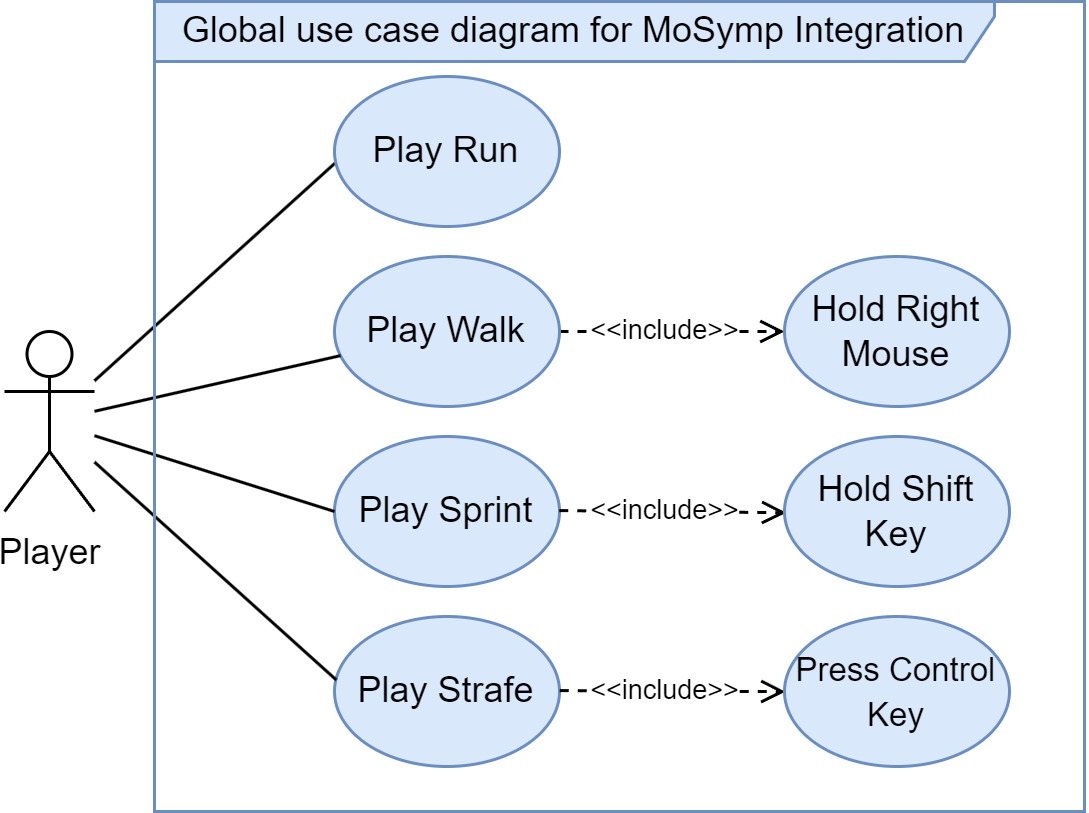
\includegraphics[scale=0.3]{Figures/uml/UserCaseMoSymp.png}}
    \caption{Global use case diagram for MoSymp Integration.}
\end{figure}\\
This diagram depicts the interactions between different player actions and the corresponding animations triggered by those actions. Player actions such as "Hold Right Mouse," "Hold Shift Key," and "Press Control Key" are represented as ellipses. The diagram illustrates the connections between these actions and specific animations like "Play Run," "Play Walk," "Play Sprint," and "Play Strafe." The arrows between the actions and animations show the relationship and sequencing of these interactions. This use case diagram visualizes how the MoSymp plugin coordinates animations based on player inputs, enhancing the gameplay experience.
\begin{figure}[!h]
    \centering
    \fbox{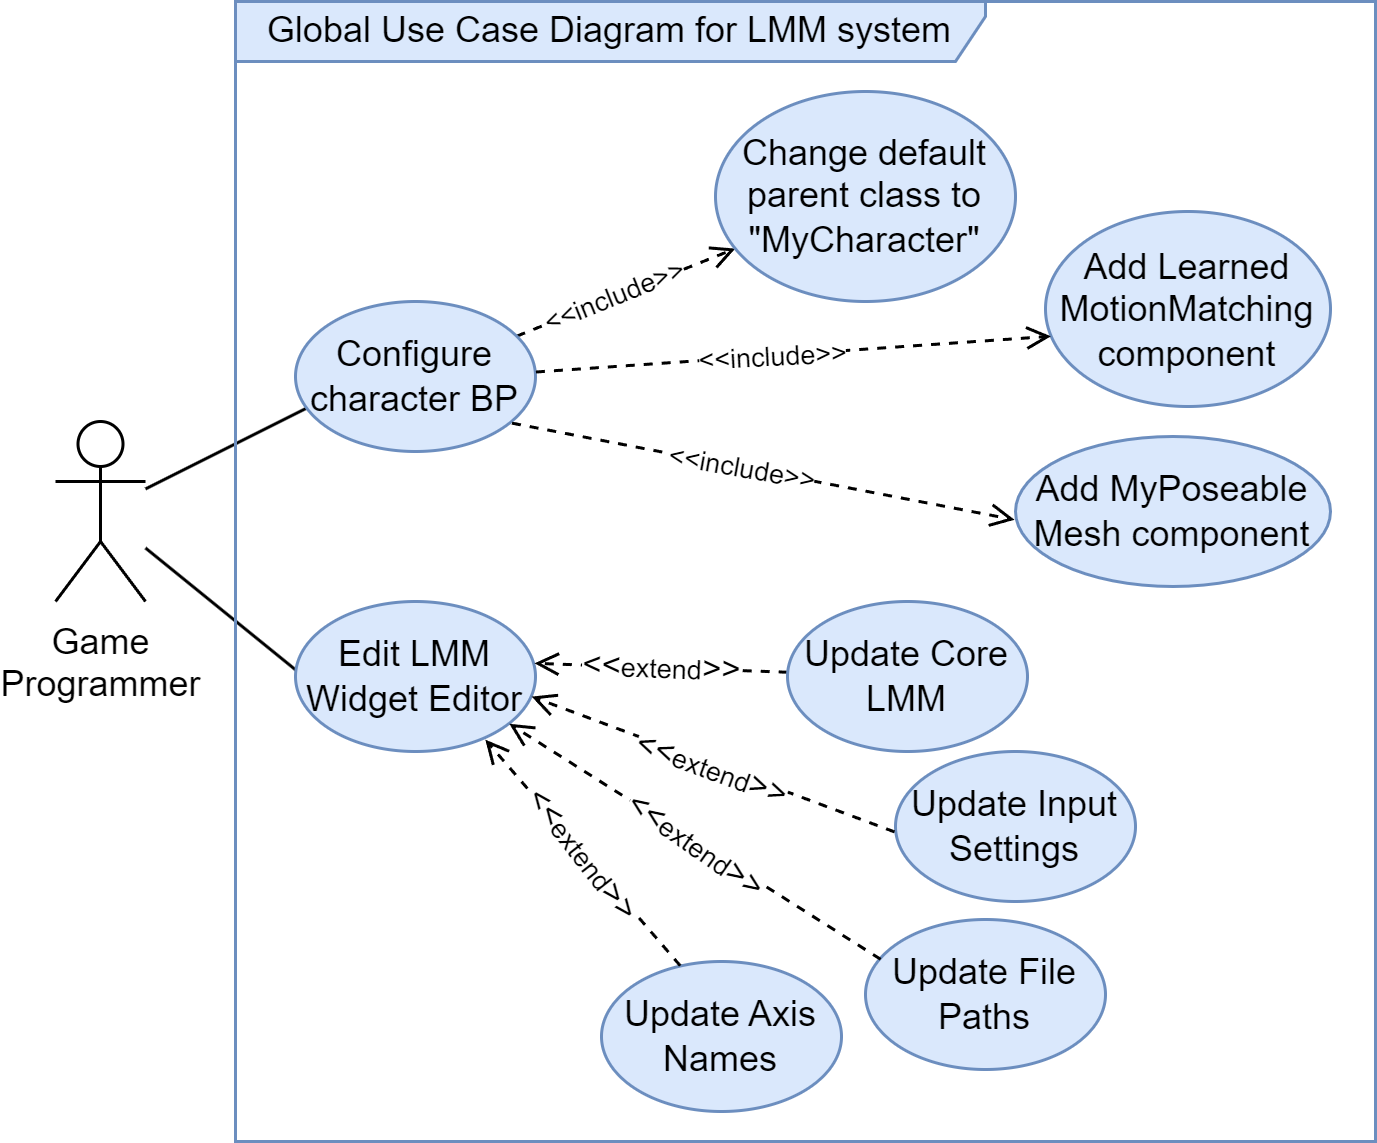
\includegraphics[scale=0.3]{Figures/uml/LMMUseCaseGlobal.png}}
    \caption{Global use case diagram for LMM}
\end{figure}
This diagram illustrates the interactions and relationships between different components and actions in the LMM system. The diagram showcases various stages of the game development process, such as configuring character blueprints, integrating motion matching components, updating input settings, and managing file paths. The use case diagram aims to provide a clear overview of how different elements of the LMM system work together to enhance character animations and gameplay experiences in game development.The system construction process will be provided in a general Class diagram and a sequence diagram of one of the system process interactions explaining the development process.
\subsection{Class diagram}
The class diagram down bellow presents the LMM system and is generally developed in a plugin format for an easy and effective integration on any character of a given game.
\begin{sidewaysfigure}
    \centering
    \fbox{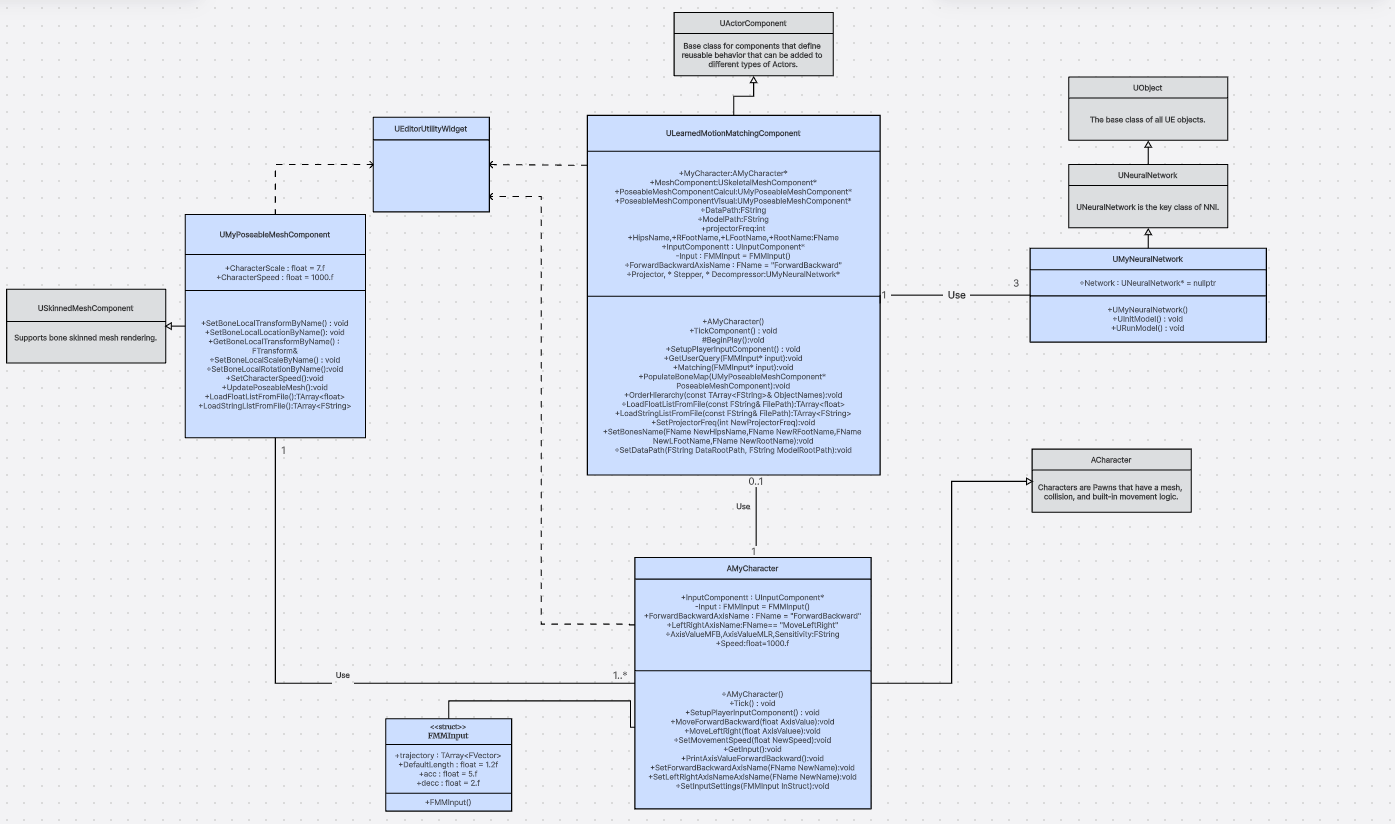
\includegraphics[scale=0.6]{Figures/uml/Class diagram LMM.png}}
    \caption{Class diagram for LMM}
\end{sidewaysfigure}

\newpage

\subsection{Sequence diagram}
This diagram presents the working of updating the MeshCompoenets in the LMM system. It explains how the user changes the parameters of the widget to update the character's Blueprint parameters and how the use of the Blueprint "Character Blueprint" is working in this case and able to present the animation result on the visual character.
\begin{figure}[!h]
    \centering
    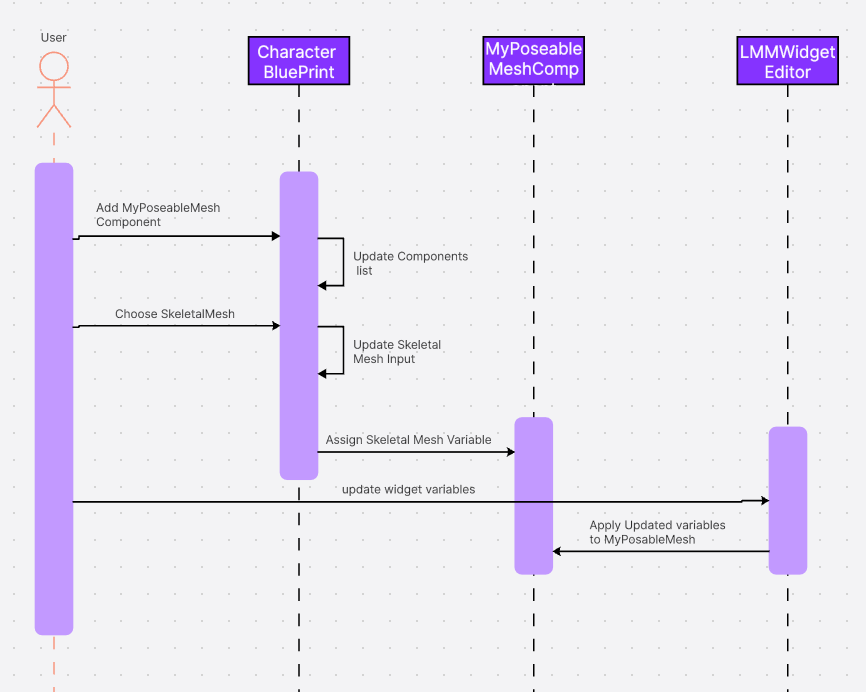
\includegraphics[scale=0.8]{Figures/uml/UpdateMeshComponent.png}
    \caption{Diagram sequance UpdateMeshComponent}
    \label{Diagram sequance UpdateMeshComponent}
\end{figure}

\newpage

\section{Internship planning:}
\begin{itemize}
    \item \underline{Training:}
          Upon the commencement of the internship, we embarked on an intensive training program
          focused on the utilization of the Unreal Engine 4 game development engine and the
          C++ language. This training was facilitated through tutorials available on the official website
          "learn.unrealengine.com" as well as YouTube resources.
    \item \underline{Conception/Design:}
          Throughout the duration of the internship, we contemplated undertaking the design phase.
          As a result, we initiated an exploration of the UML language, a fundamental design language,
          utilizing the "Draw.io" software as our tool of choice.
    \item  \underline{Development:}
          The development phase commenced with a slight delay, as previously mentioned in the
          self-study section. During this phase, we employed the Unreal Engine 5 to seamlessly integrate
          and refine the new system, incorporating all its intricate aspects and adjustments. This
          comprehensive implementation aimed to optimize its utility for future production purposes,
          facilitating the work of fellow developers and animators.
    \item  \underline{Realization of the report: }
          We commenced the report writing process in early May and successfully completed it
          within the initial days of June.
    \item \underline{Appliance of the system:}
          We dedicated a period of over two and a half months to the implementation and
          advancement of our modified system.
\end{itemize}

\section{Conclusion:}
In this chapter, we have provided a concise overview of the project at hand, outlining the
identified problem and proposing a solution to address the current situation.

%-------------------------------------------------------------------------------------------------------
\begin{ConfigureChapter}
    \chapter{\textbf{Realisation}}
    \minitoc
\end{ConfigureChapter}
%-------------------------------------------------------------------------------------------------------
\fancyhead[R]{Realisation}
\newpage

\section{Introduction}
\lettrine[findent=1pt]{\textbf{T}}{his} chapter represents the last part of this report, it is devoted to the implementation aspect and to the presentation of the work carried out. We start with the architectures used and the development software environments. Thereafter, we illustrate the functionalities developed with some screenshots presenting the interfaces carried out
\section{Work environment:}
Within this section, we will explore the active implementation of work processes at Lanterns Studio.
\subsection{Workflow in Lanterns Studio:}
At the beginning of each week, every team holds a meeting where they collectively review tasks from the current and previous weeks.
This gathering aims to address any ambiguities or challenges that may have arisen. Seniors actively support interns and junior team members
with their upcoming tasks. During these meetings, developers openly express their genuine opinions regarding the gameplay, while seniors engage in testing the game firsthand to provide valuable feedback and reviews.
For Tasks Management Lanterns Studio uses ClickUp.
\begin{figure}[!h]
    \centering
    
\includegraphics[scale=0.03]{./Figures/Images/ClickUp-Logo.png}
    \caption{ClickUp Logo}
    \label{ClickUp Logo}
\end{figure}\\
Similar to popular tools such as Trello and Jira, ClickUp is a software solution that empowers companies to efficiently manage their workflow using features like whiteboards, BurnDown Charts, and more.
\begin{figure}[!h]
    \centering
    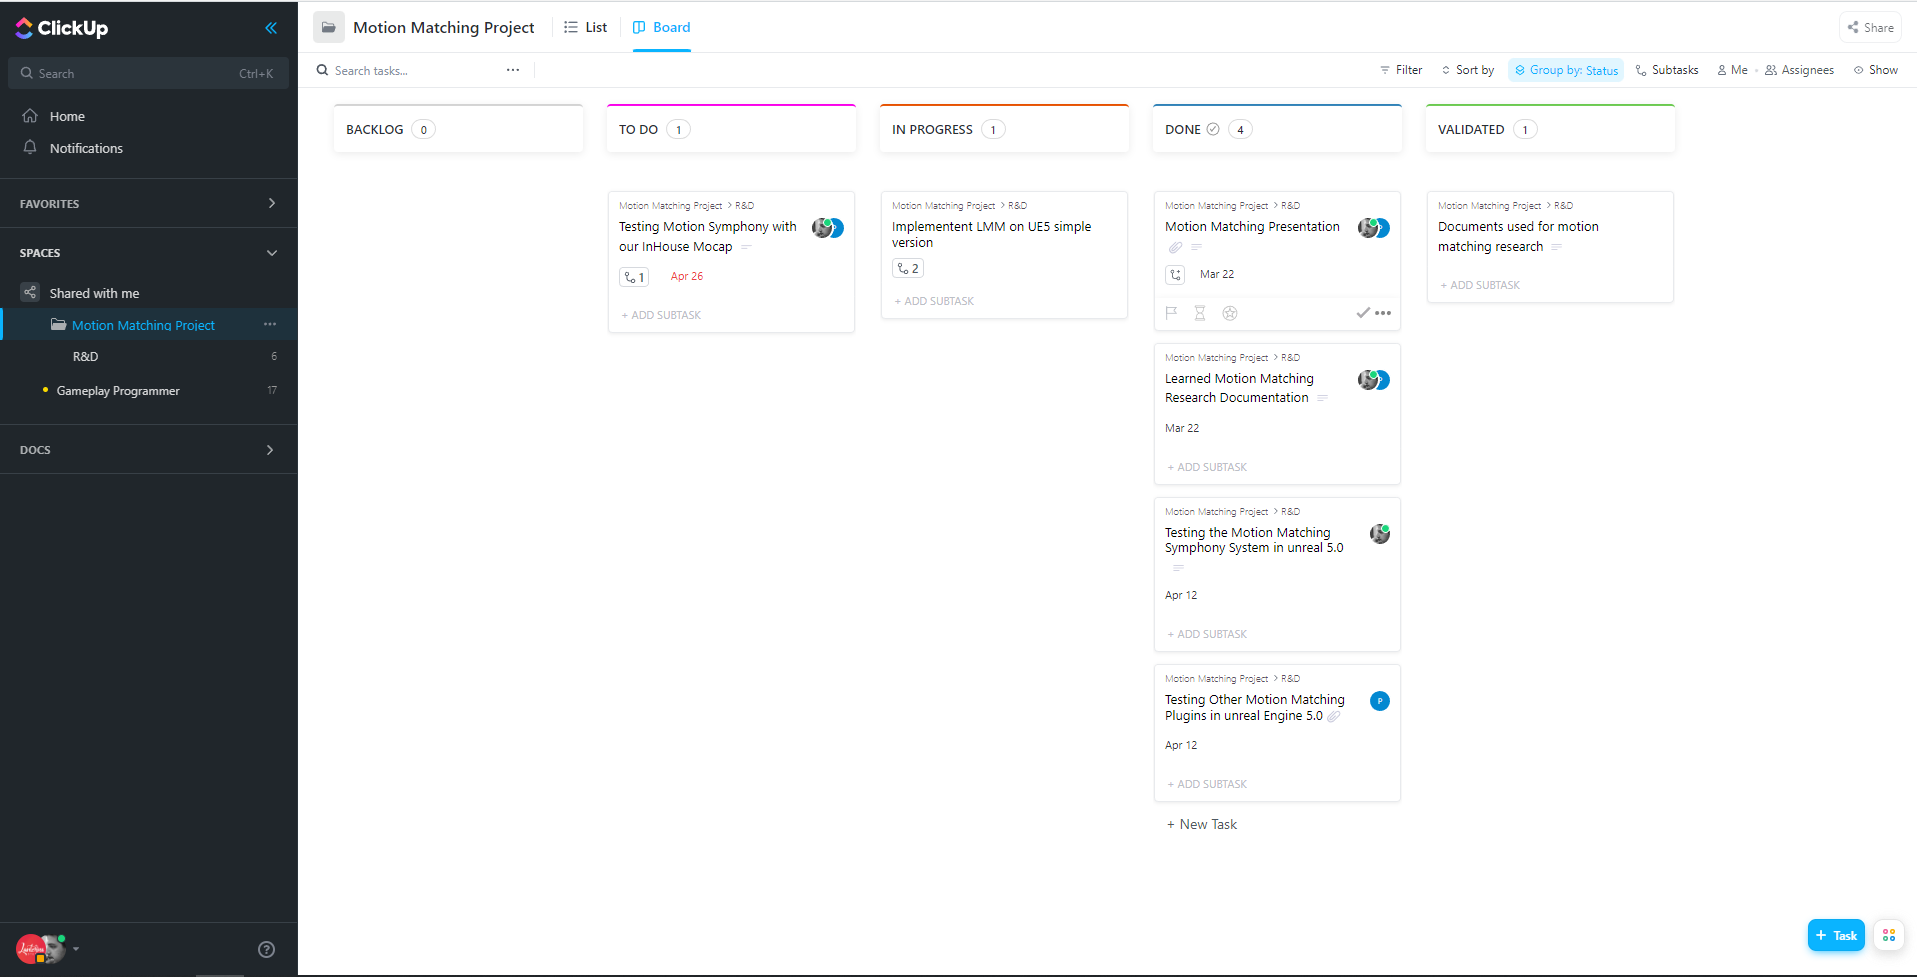
\includegraphics[scale=0.35]{./Figures/Images/ClickUp whiteboard.png}
    \caption{ClickUp whiteboard}
    \label{ClickUp whiteboard}
\end{figure}\\
The whiteboard showcases various columns, ranging from backlog to validated, providing an organized arrangement of tasks with assigned start dates and deadlines. Tasks are initially placed in the backlog, and individuals are responsible for managing their own tasks based on their current status. Upon completion, the task undergoes evaluation by the mentor or team director, who either validates it or requests revisions if necessary.
\newpage

\section{Development tools}
\subsection{Unreal engine}
Unreal Engine, abbreviated as UE, stands as a prominent 3D computer graphics game engine developed by Epic Games.
Its debut was marked by the unveiling of a first\-person shooter titled Unreal. Initially tailored for PC FPS games,
Unreal Engine expanded its scope to encompass diverse game genres, and later found applications in other industries like film,
television, and movies. Developed in C++, the engine boasts extensive portability, supporting a wide range of platforms,
including PlayStation, Xbox, Nintendo consoles, as well as mobile, desktop, and virtual reality platforms.
Over the years, Unreal Engine has garnered immense acclaim, powering highly acclaimed games like Tekken 7 (2015), BioShock (2007),
its sequel in 2010, and numerous others. The latest version, UE5, witnessed a significant adoption by companies due to its hyper\-realistic graphics fueled by the Nanite
feature and life\-like lighting effects enabled by the Lumin feature.
\begin{figure}[!h]
    \centering
    
\includegraphics[scale=0.05]{./Figures/Images/unreal.png}
    \caption{Unreal engine 5}
    \label{Unreal engine 5}
\end{figure}

\newpage

\subsection{Visual studio}
Visual Studio is a comprehensive integrated development environment (IDE) designed by Microsoft. It caters to a wide range of programming languages and platforms, offering advanced tools and features for efficient software development. With its user-friendly interface and powerful debugging capabilities, Visual Studio provides developers with a seamless and productive coding experience. It remains a go-to choice for professionals and beginners alike, empowering them to build, test, and deploy applications with ease and precision.
\begin{figure}[!h]
    \centering
    
\includegraphics[scale=0.03]{./Figures/Images/Visual-Studio-logo.png}
    \caption{Visual studio}
    \label{Visual studio}
\end{figure}

\subsection{ONNX and NNE}
ONNX is an open format built to represent machine learning models. ONNX defines a common set of operators - the building blocks of machine learning and deep learning models - and a common file format to enable AI developers to use models with a variety of frameworks, tools, runtimes, and compilers.
\begin{figure}[!h]
    \centering
    
\includegraphics[scale=0.3]{./Figures/onnx-stacked-color.png}
    \caption{ONNX technology}
    \label{ONNX technolofie}
\end{figure}
\begin{figure}[!h]
    \centering
    
\includegraphics[scale=0.7]{./Figures/NNE.png}
    \caption{ONNX NNE plugin}
    \label{ONNX NNE plugin}
\end{figure}
NNE is a platform to run pre-trained neural network models inside games. It supports both CPU and GPU inference on desktop machines and on some consoles. The plugin serves as an abstraction layer for various runtimes with each runtime targeting specific hardware.

The core asset in NNE is UNNEModelData which stores the data of a neural network model. It can be passed in-game to either a runtime implementing INNERuntimeCPU to create a CPU model IModelCPU or to a runtime implementing INNERuntimeRDG to create a model IModelRDG which can be used for GPU inference.
To use NNE, the core plugin has to be enabled as well as all the plugins of the different runtimes needed.

\subsection{PyTorch}
PyTorch is an open-source deep learning framework that has gained widespread popularity among
researchers and developers alike. Known for its flexibility and ease of use, PyTorch enables
efficient creation and training of complex neural networks. It utilizes dynamic computation
graphs, which make it easier to debug and experiment with models. PyTorch also supports
automatic differentiation, allowing gradients to be calculated effortlessly, crucial
for optimizing model parameters during training. Its Python-first approach and extensive
documentation foster a welcoming community and facilitate seamless integration with various
Python libraries. As a result, PyTorch has become a preferred choice for researchers,
educators, and AI practitioners seeking a powerful and intuitive framework for their deep
learning projects.
\begin{figure}[!h]
    \centering
    
\includegraphics[scale=0.2]{./Figures/Images/Pytorch_logo.png}
    \caption{PyTorch}
    \label{Pytorch}
\end{figure}

\subsection{Maya}
Maya is professional 3D software for creating realistic characters and blockbuster-worthy effects.
It bring believable characters to life with engaging animation tools and Shape 3D objects and scenes with intuitive modeling tools with the Creation of realistic effects—from explosions to cloth simulation.
\begin{figure}[!h]
    \centering
    
\includegraphics[scale=0.08]{./Figures/Images/maya.png}
    \caption{Maya}
    \label{Maya}
\end{figure}

\subsection{Cpp}
C++ serves as the primary programming language for Unreal Engine, offering developers a powerful and efficient toolset to create sophisticated games and interactive experiences. With its robust capabilities and low-level access to engine features, C++ enables precise control and optimization, allowing developers to fine-tune performance for their projects. Unreal Engine's C++ support ensures seamless integration with its visual scripting system, Blueprint, facilitating a flexible and hybrid development approach. As a widely-used and industry-proven language, C++ empowers developers to unleash their creativity and build immersive worlds within the Unreal Engine ecosystem.
\begin{figure}[!h]
    \centering
    
\includegraphics[scale=0.04]{./Figures/Images/cpp.png}
    \caption{Visual studio}
    \label{Visual studio}
\end{figure}

\subsection{Python}
Python for Unreal (PyUnreal) is a powerful integration that enables developers to leverage Python scripting within the Unreal Engine
environment. This seamless combination empowers users to automate tasks, create custom tools, and extend functionality in Unreal
Engine with the ease and flexibility of Python. With PyUnreal, developers can streamline workflows, prototype rapidly, and enhance
productivity, making it an invaluable addition to Unreal Engine's arsenal of development tools.
\begin{figure}[!h]
    \centering
    \includegraphics[scale=0.04]{./Figures/Images/Python.png}
    \caption{Python}
    \label{Python}
\end{figure}

\subsection{Csharp}
Csharp (pronounced "See Sharp") is a modern, object-oriented, and type-safe programming language. Csharp enables developers to build many types of secure and robust applications that run in .NET. Csharp has its roots in the C family of languages and will be immediately familiar to C, C++, Java, and JavaScript programmers. This tour provides an overview of the major components of the language in Csharp 11 and earlier.
\begin{figure}[!h]
    \centering
    
\includegraphics[scale=0.3]{./Figures/Images/csharp.png}
    \caption{Csharp}
    \label{Csharp}
\end{figure}

\newpage

\section{Training courses}
In this section, we'll present the internship curriculum training with the UE5 environment.
For about 2 months, the Lanterns training for the game development industry is quite complex specially for AAA game production. That's why some essential basics must be taken in considerations. Down bellow we provide the list of courses needed to complete before fully immerse ourselves in the project research and development.
\begin{figure}[!h]
    \centering
    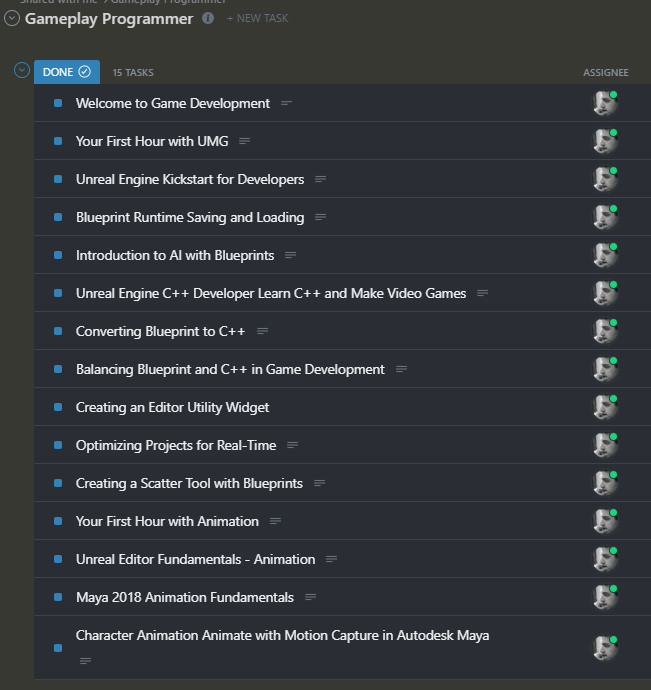
\includegraphics[scale=0.7]{./Figures/formation.png}
    \caption{Training courses in UE5}
    \label{Training courses in UE5}
\end{figure}
\newpage
\section{Implementation of Motion Symphony}
\subsection{Introduction} 
\lettrine[findent=1pt]{\textbf{I}}{n} this section, we showcase a prototype that leverages the MoSymph system in conjunction with recorded MoCap data using the research results in the annex section \ref{appendix:MS}.

\subsection{Recorded Animations}
In this prototype, we incorporated a variety of recorded Mocap animations, which were categorized based on their types of movement and shown in the figure 3.13 down bellow.

\begin{sidewaysfigure}
    \centering
    \fbox{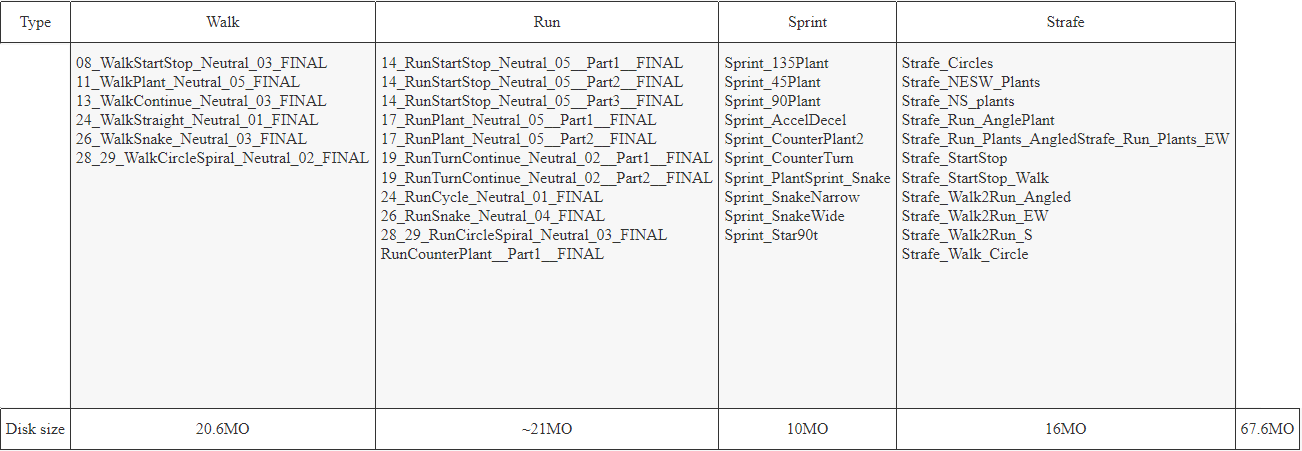
\includegraphics[scale=0.6]{Figures/Images/AnimationTable.png}}
    \caption{MoCap aniamtions used in our prototype.}
    \label{tab:my_label}
\end{sidewaysfigure}

\subsection{Implementation}

When working with MoCap animations, it is necessary to clean the animations to meet specific standards, ensure comprehensive coverage, optimize data search during runtime, and achieve a cohesive and consistent animation result.\newline
To achieve this process, we utilize a Tag System with a try and catch mechanism. The successful execution of this system relies on comprehending the concepts explained in the research section. For instance, in the following example, we apply a low CostMultiplier Tag to a walk cycle, prioritizing its playback and avoiding interruptions from similar poses.

 \begin{figure}[!h]
    \centering
     \fbox{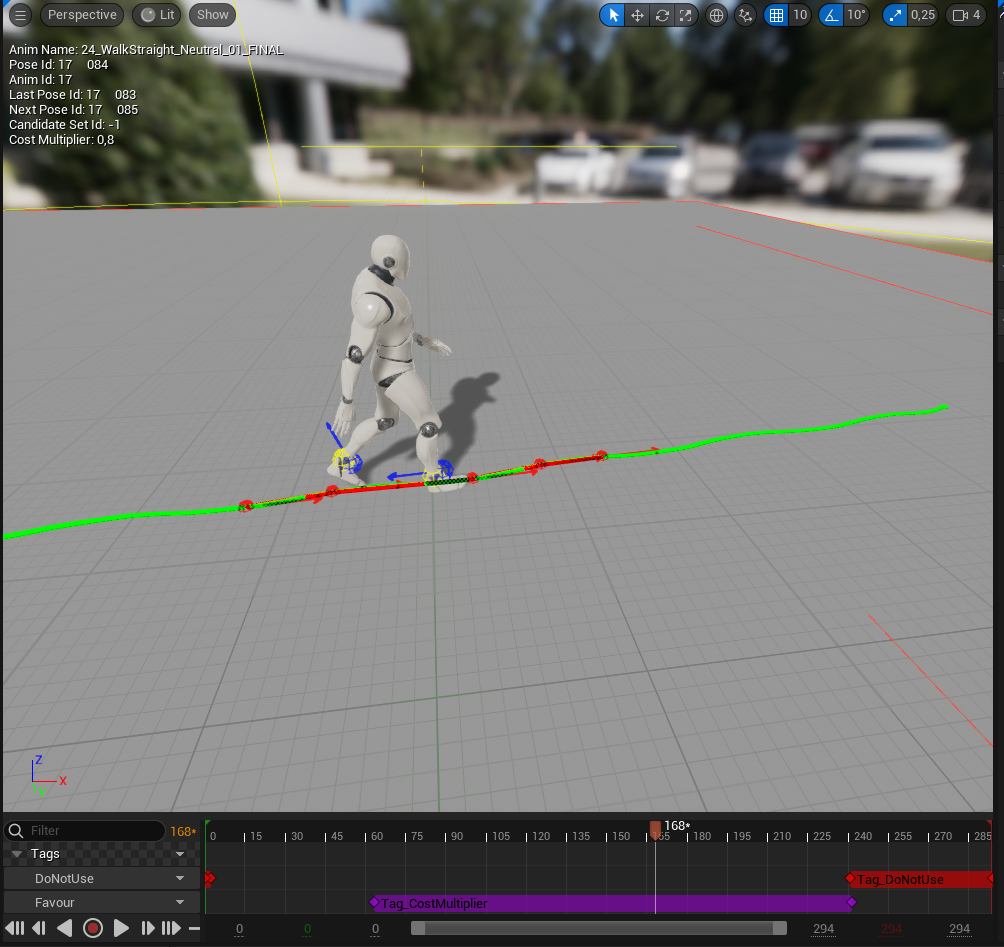
\includegraphics[scale=0.3]{Figures/Images/AnimationTagWalkStraight_Neutral.png}}
    \caption{WalkStraight\_Neutral animation Tag.}
   \end{figure}
To animate the character, it is essential to establish a logical connection between the various movement types of the character. This allows us to switch between different data assets based on the player's input.  

\begin{figure}[!h]
    \centering
    \fbox{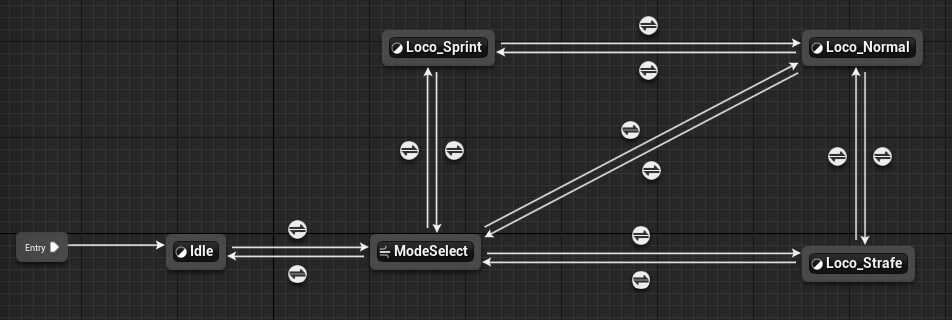
\includegraphics[scale=0.5]{Figures/Images/StateMachines.png}}
    \caption{Relations between state machines in the animation Blueprint.}
   \end{figure}
Once the character's state machine is set up, the next step involves creating and configuring the appropriate mechanical logic for player movement. This logic encompasses several aspects: controlling the camera, managing animation inputs (such as strafing, walking, and sprinting), implementing trajectory error correction, generating motion-matching trajectories, and aligning the trajectory generator's strafe direction with respect to the camera orientation.
   \begin{figure}[!h]
    \centering
     \fbox{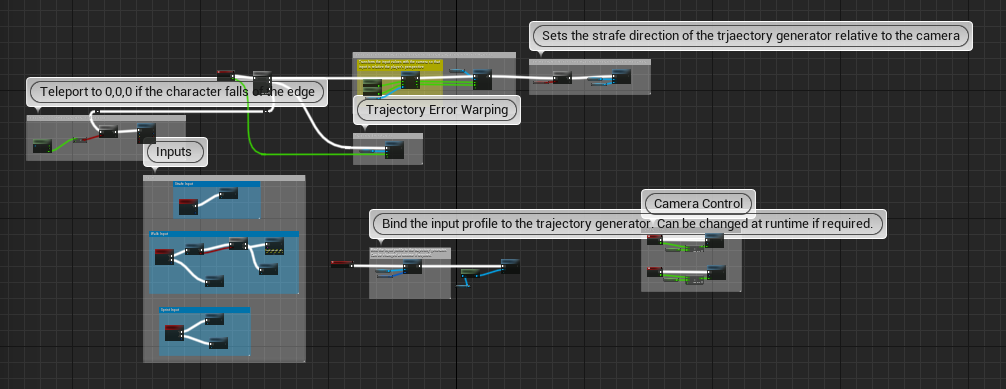
\includegraphics[scale=0.5]{Figures/Images/BP_MotionMatchingCharacter.png}}
    \caption{Character Blueprint.}
   \end{figure}

Similar to the Blueprint of the player character, we set up its animation blueprint to retrieve the accurate trajectory information from the trajectory generator component attached to the player character. The rest of the logic serves the purpose of managing state transitions and should be tailored to align with the character's specific movements.
 \begin{figure}[!h]
    \centering
     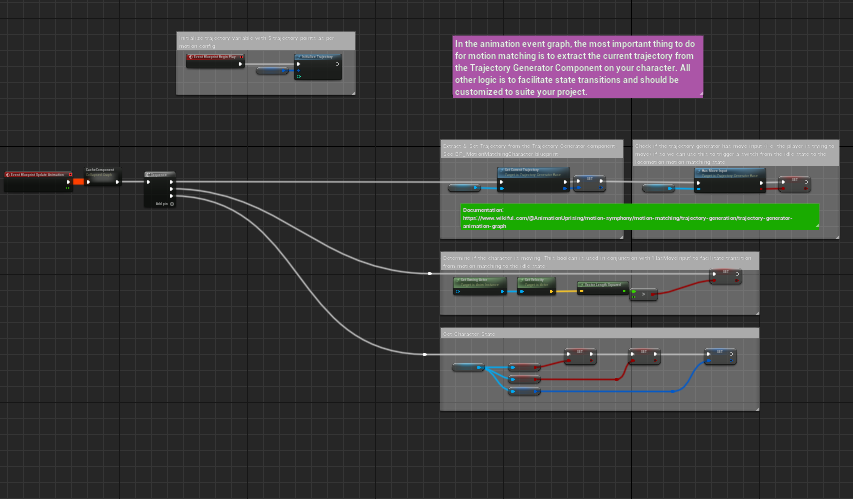
\includegraphics[scale=0.5]{Figures/Images/demo event graph MS.png}
    \caption{Event graph of the Animation Blueprint.}
   \end{figure}
\newpage
   \begin{figure}[!h]
    \centering
     \fbox{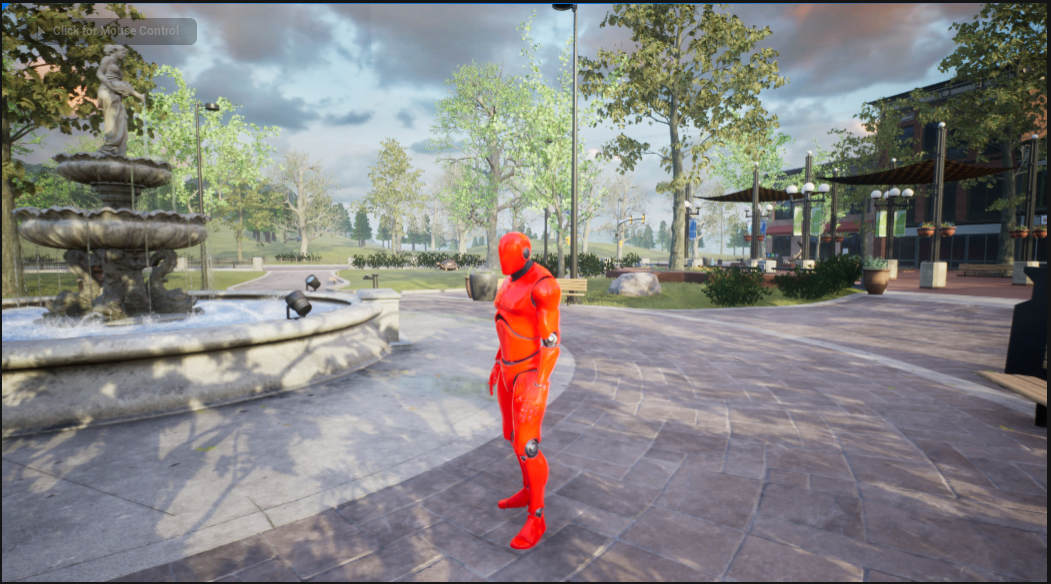
\includegraphics[scale=0.5]{Figures/Images/demo.png}}
    \caption{Player Character implemented in the level.}
   \end{figure}
We lastly need to configure our project's "GameMode" to make the player character's Blueprint spawn in our level as the default Pawn Class and try to visualize its movements.

\newpage

\section{Learned Motion Matching}
\lettrine[findent=1pt]{\textbf{I}}{n} this section, we'll implement the Learned motion matching mechanics and throw applying the research results in the annex section \ref{appendix:LMM}, the steps needed to successfully implement it are presented bellow.
\newpage
\subsection{The machine learning process}
the figure bellow sows the process of generating the ONNX files after training the python models of the decompressor,
\begin{figure}[!h]
    \centering
     \fbox{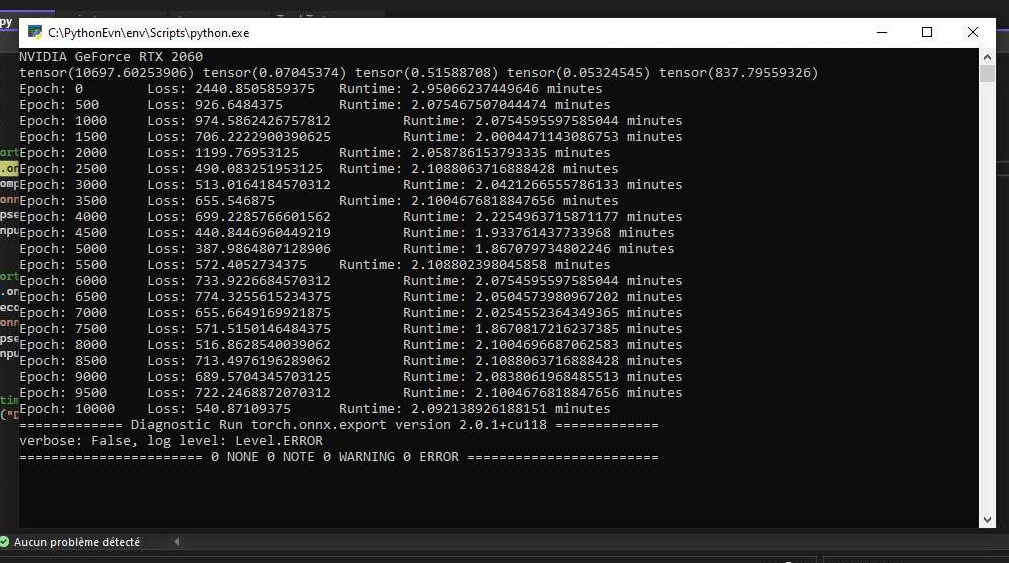
\includegraphics[scale=0.6]{Figures/LearningProcessPythorch.png}}
    \caption{the machine learning process.}
\end{figure}

\subsection{Implementing "MyNeuralNetwork" object}
Creating a mechanism to invoke models dynamically during runtime is fundamental, which we accomplish within the UMyNeuralNetwork class by two main functions UInitModel and URunModel.

   \begin{figure}[!h]
    \centering
     \fbox{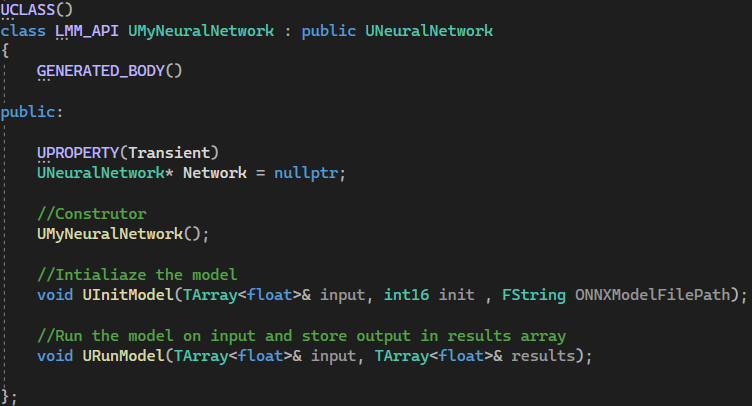
\includegraphics[scale=0.6]{Figures/Images/UMyNeuralNetwork.png}}
    \caption{MyNeuralNetwork header.}
   \end{figure}
   
\subsection{Implementing "MyPoseableMeshComponent" component}
The class "MyPoseableMeshComponent" enables real-time manipulation of bones, facilitating tasks such as retrieving and modifying their positions and orientations. Including it within the character Blueprint is a necessary step due to its custom nature as a component.  

 \begin{figure}[!h]
    \centering
     \fbox{
\includegraphics[scale=0.7]{Figures/Images/AddMyPoseableMeshC.png}}
    \caption{Add "MyPoseableMeshComponent" to CharacterBP.}
   \end{figure}

The following code snippet illustrates how we dynamically modify the position of the root bone during runtime.

  \begin{figure}[!h]
    \centering
     \fbox{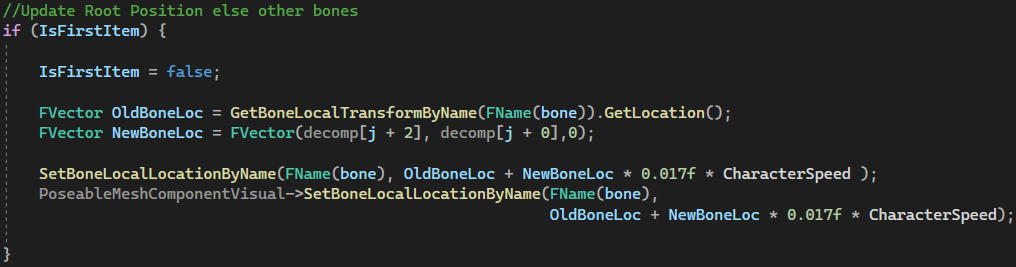
\includegraphics[scale=0.6]{Figures/Images/UpdatePositions.png}}
    \caption{Update Root bone location.}
   \end{figure}

\subsection{Implementing "MyCharacter" actor}

We found it imperative to modify the built-in "ACharacter" class. This adaptation was crucial for introducing new axis bindings, thereby enabling us to capture and interpret user input according to our defined parameters.

  \begin{figure}[!h]
    \centering
     \fbox{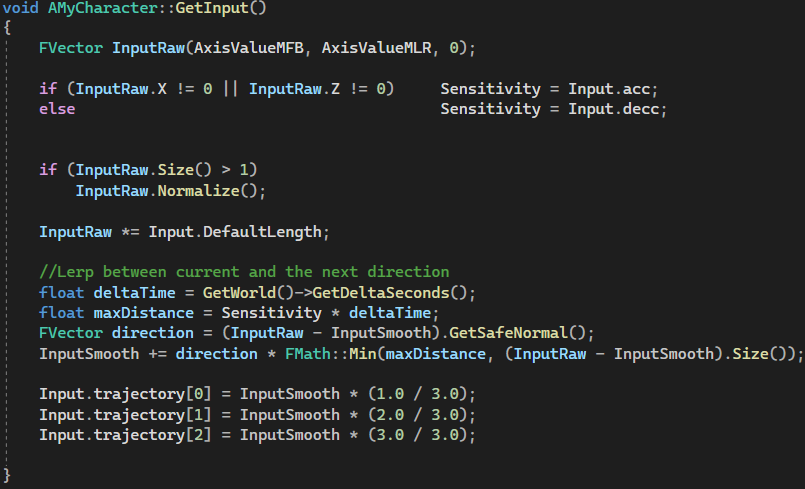
\includegraphics[scale=0.6]{Figures/Images/GetInput.png}}
    \caption{Update Character's input.}
   \end{figure}

The following figure shows the action of selecting "MyCharacter" as the primary parent class for our character Blueprint. 

  \begin{figure}[!h]
    \centering
     \fbox{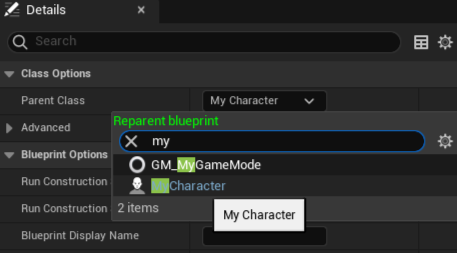
\includegraphics[scale=0.6]{Figures/Images/ParentClass.png}}
    \caption{Set characterPB parent class.}
  \end{figure}
  
\subsection{Implementing "LearnedMotionMatchingComponent"}
At the heart of our system lies this fundamental class, responsible for orchestrating the reception of fresh queries and then passing them to our models. This strategy is in harmony with the Projector-Stepper-Decompressor concept that has been elucidated in the state of the art and research section. The following figure shows a part of the GetQuery.
 \begin{figure}[!h]
    \centering
     \fbox{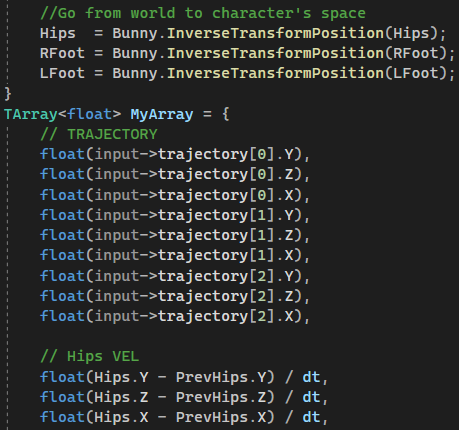
\includegraphics[scale=0.6]{Figures/Images/GetQuery.png}}
    \caption{Get trajectory points and Hips velocity.}
   \end{figure}

Adding the "LearnedMotionMatchingComponent" to the character Blueprint is a necessary step, much like including the "MyPoseableMeshComponent".

\begin{figure}[!h]
    \centering
     \fbox{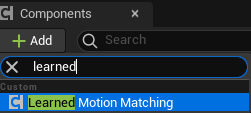
\includegraphics[scale=0.7]{Figures/Images/AddLMMC.png}}
    \caption{Add "LearnedMotionMatchingComponent" to CharacterBP.}
   \end{figure}

\subsection{Implementing Widget Editor Utility}
In order to facilitate the configuration of variables for users of our system, we are introducing the Learned Motion Matching Widget Editor Utility. This Blueprint enables users to customize a variety of variables, all without requiring access to Cpp code or involvement in the compilation process. The following figure shows the design of our widget.

\begin{figure}[!h]
    \centering
     \fbox{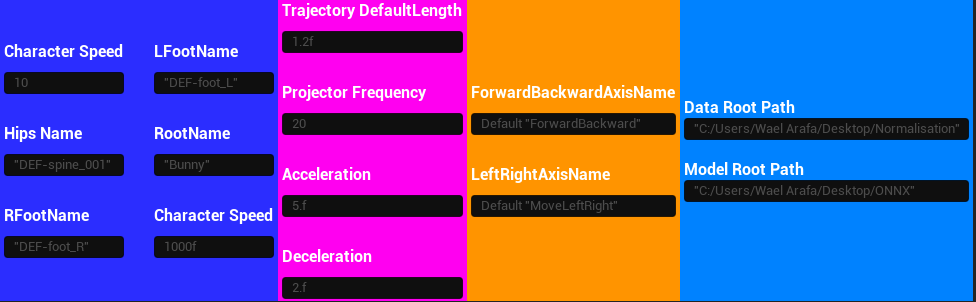
\includegraphics[scale=0.4]{Figures/Images/Widget.png}}
    \caption{Widget Editor Utility Design.}
\end{figure}
\newpage
\begin{figure}[!h]
    \centering
     \fbox{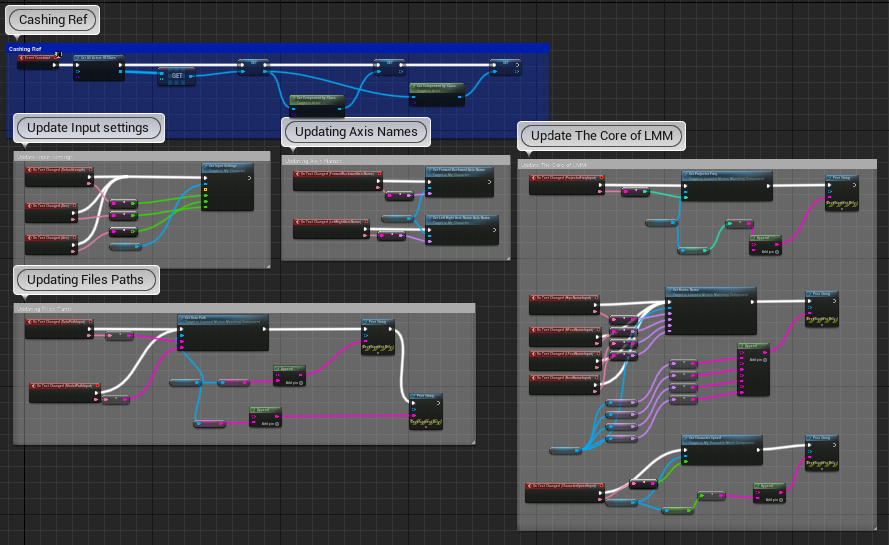
\includegraphics[scale=0.5]{Figures/Images/WidgetBluePrint.png}}
    \caption{Widget Editor Utility Blueprint.}
\end{figure}
The process of assigning values to variables within Blueprints from Cpp code involves utilizing a series of nodes, which are depicted in the next figure..

\newpage
\section{Statistics comparison}
\lettrine[findent=1pt]{\textbf{I}}{n} this section, we'll show bellow the different  between both the MS (figure 3.29) and the LMM (figure 3.30) in some statistics results shown in the unreal engine 5 metrics. 
\begin{figure}[!h]
    \centering
     \fbox{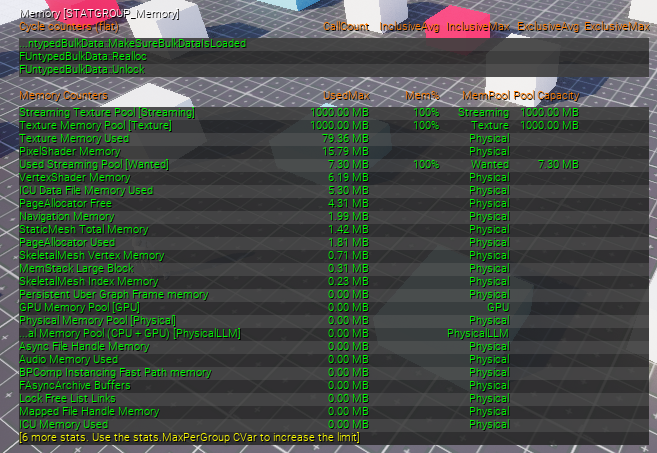
\includegraphics[scale=0.8]{Figures/memory statistics MS.png}}
    \caption{Motion Symphony memory stats.}
\end{figure}
\begin{figure}[!h]
    \centering
     \fbox{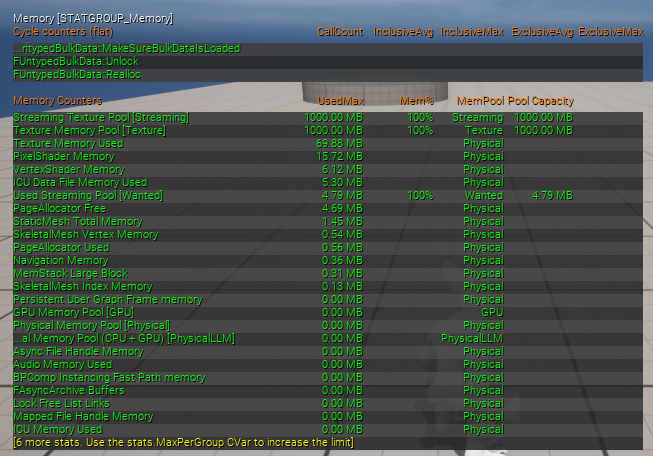
\includegraphics[scale=0.9]{Figures/memory statistics lmm.png}}
    \caption{LMM memory stats.}
\end{figure}
The stat memory command provide us in UE5 the possibility to profile the project's memory use (by milliseconds) in the engine and allow us to visualise the difference in our case between both the motion symphony solution and the LMM solution developed and precisely see the difference between both. In this case, we can visualise the difference in the "used streaming pool", the "Skeletal Mesh Index Memory" and the "Navigation Memory".
\section*{Conclusion}
In this chapter, we presented the environment on which was carried out, the steps of development then we specified the indicators of the quality of the solution. Finally, we exposed captures of the different interfaces to give a better idea about our project.
\newpage
%-----------------------------------------------------------------------------------------------
\begin{ConfigureChapter}
    \chapter{\textbf{General Conclusion and perspectives}}
    \mtcaddchapter{}
\end{ConfigureChapter}
%-----------------------------------------------------------------------------------------------
In conclusion, the adoption of Learned Motion Matching technology represents a pivotal advancement in game development. This technology addresses the limitations of traditional animation techniques by leveraging machine learning algorithms to synthesize realistic and dynamic character movements in real-time. The benefits are multifaceted: it streamlines animation creation, reduces development costs, and enhances player immersion by ensuring smooth and responsive animations. This technology offers a dynamic solution adaptable to various scenarios, freeing developers from the constraints of manually creating countless animations. Games incorporating this technology exhibit enhanced realism, responsiveness, and adaptability, creating immersive player experiences. Furthermore, industry giants like Epic Games, Ubisoft, and EA Sports have embraced Learned Motion Matching, demonstrating its feasibility potential. As this technology continues to evolve, it stands to reshape how game developers approach animation, paving the way for richer, more engaging gaming worlds and experiences.\\
To further improve the project's quality, we can in a future aspect of the system, implement the learning process of more complex animations (the generic type of animations), making it able to generate realistic animations of animal base characters or heavy mechanical ones without consuming more memory space that it should and gaining more realistic visuals.   

\appendix 
\begin{ConfigureChapter}
    \chapter{\textbf{Research's results Annex}}
    \minitoc
\end{ConfigureChapter}
\fancyhead[R]{State of art and Research}

\lettrine[findent=1pt]{\textbf{I}}{n} this annex, we present all the research results, including the animation workflow and the motion matching scientific concept, the motion matching system, the motion symphony configurations and the LMM's concept.      

\label{appendix:state}
\section{prerequired knowledge:}
\label{appendix:state}
\lettrine[findent=1pt]{\textbf{I}}{n} this section, we'll present the animation system that most of the game engines work by and will explain the technical notations about each one. 
\subsection{Animation Clips:}
movement and actions in characters or objects within a game or animation. The
classification of animation clips encompasses three primary types: \textbf{cycles}, \textbf{actions}, and
\textbf{transitions}. The categorization is not solely based on the nature of the action itself but also takes
into account the initiation and conclusion of the animation.
\begin{itemize}
    \item \textbf {Cycles : }they are animations that can repeat indefinitely, such as a character's walking or running animation.
          \begin{figure}[h!]
              \centering
              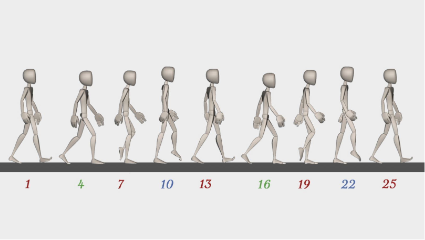
\includegraphics[scale=1]{Figures/Images/walk cycle animation exemple.PNG}
              \caption{Walk cycle}
          \end{figure}
    \item \textbf {Actions : }they are animations with a clear start and end point, such as a character's attack animation.
          \begin{figure}[h!]
              \centering
              \includegraphics[scale=1]{Figures/Images/attack action exemple.png}
              \caption{Attack Action}
          \end{figure}
    \item \textbf {Transitions : }are animations that connect two other animations together, such as a character transitioning from their idle animation to their running animation.
\end{itemize}
There are two main approaches to create animation clips :
\begin{itemize}
    \item \textbf{Key frame Animation Clips :}
          these clips define the animation by specifying a series of keyframes, where each key frame represents a particular point in time
          and position of an object or character. The computer then fills in the gaps between keyframes to create a smooth animation.
    \item \textbf{Motion Capture Animation Clips :}
          these clips use data captured from real-world motion capture sessions to animate characters and objects in the game.
          This technique involves recording the movements of actors wearing motion capture suits or markers and then mapping that data
          onto a digital character model. The resulting animation clip is highly realistic and captures subtle nuances of human movement.
\end{itemize}
\subsection{Skeletal rig}
In computer graphics and animation, we often utilize a skeletal representation that consists of interconnected joints (depicted in Figure 1.4).
These joints serve as counterparts to the articulated parts of the human body. Each vertex of the mesh is linked to one or multiple joints, and any movement made by a joint results in a corresponding movement of the associated vertices.
\begin{figure}[!h]
    \centering
    \includegraphics[scale=0.4]{./Figures/Images/Representation of a humanoid skeleton.png}
    \caption{Representation of a humanoid skeleton. (Spheres represent joints)}
    \label{Representation of a humanoid skeleton. (Spheres represent joints)}
\end{figure}

\subsection{State Machines:}
State machines are a variant of behavior nets, encompassing a collection of states or
actions, transitions, and an entry point. The states within the state machine denote specific
activities, while the transitions outline the process of transitioning between these activities.
Traffic lights serve as an illustrative instance of a state machine, where circles represent states,
arrows denote transitions, and specific conditions trigger these transitions. The states represent activities, and transitions represent how to switch between them [Hofkamp 2015] \cite{url-4}.
\begin{figure}[h!]
    \centering
    \includegraphics[scale=0.5]{./Figures/Images/Traffic light state machine.PNG}
    \caption{Traffic light state machine}
    \label{Traffic light state machine}
\end{figure}

\subsection{Blending:}
Animation blending, as a concept, simply means making a smooth transition between two or
more animations on a single character or Skeletal Mesh \cite{url-5}.
\begin{figure}[h!]
    \centering
    \includegraphics[scale=0.7]{./Figures/Images/Blending.jpg}
    \caption{Process of blending}
    \label{Process of blending}
\end{figure}

\section{Motion Matching research results:}
\label{appendix:MM}
\lettrine[findent=1pt]{\textbf{B}}{y} employing motion matching, game developers can
create immersive and lifelike worlds that respond to player actions while streamlining development time and costs.

\subsection{Basic Motion matching:}
\subsubsection{\underline{\textbf{I. Trajectory:}}}
\begin{itemize}
    \item \underline{Trajectory prediction:}
          During runtime, creating the desired trajectory is a part of gameplay programming. It can be accomplished by collecting samples over a time horizon, without factoring in the current momentum of the character.
          If we assume a constant linear velocity of 1 unit per sample, starting at position 5 and with a speed of 10 units per sample, the resulting trajectory over 4 samples would be:
          
          $$
              Sample 1:\;\;\;\;Position = Starting \;position + Velocity * Time = 5 + 0 * 1 = 5$$
          $$...$$
          $$  the \;resulting \;trajectory \;over \;4 \;samples \;would \;be \;5, \;15, \;25 \;and \;35.
          $$\\
          To account for momentum, the sampling process will involve the use of the linear velocity
          and a smoothing function like an exponential decay function for acceleration and deceleration.
          Figure 4.10 presents the code that implements this function, which interpolates between the
          current value and the target value.
    \item \underline{Inverse transforming trajectories:}
          In order to generate the intended path of a character, the trajectory is initially created in
          world space. However, it needs to be converted back into the animation or global space, which
          represents the character’s position and orientation at the beginning of the animation. This
          conversion is accomplished by multiplying each point of the trajectory by the inverse of the
          animation transform.
          \begin{figure}[!h]
              \centering
              \includegraphics[scale=0.5]{./Figures/Images/InverTT.jpg}
              \caption{Transforming the desired trajectory.}
              \label{Transforming the desired trajectory.}
          \end{figure}\\
    \item \underline{Trajectory curves matching:}
          Calculating the distance between each sample point on the desired trajectory and its equivalent
          point on the cached trajectories is necessary when comparing a desired trajectory to all of the
          previously cached once. The ultimate cost, which serves as an indicator of how well the planned
          trajectory matches the cached ones, is calculated by adding up these distances. The more The
          desired trajectory and the stored trajectories match up the lower the cost is.
          \begin{figure}[!h]
              \centering
              \includegraphics[scale=0.7]{./Figures/Images/TrajectoryMatch.jpg}
              \caption{Matching trajectories}
              \label{Matching trajectories}
          \end{figure}\\
          Trajectory-matching is used to select an animation pose that closely aligns with the desired
          trajectory, but it may not necessarily result in realistic human locomotion. To achieve high-
          quality animation motion, the focus shifts to selecting animations with a similar pose to the
          currently playing one, prioritizing animation quality over input responsiveness.
    \item \underline{Past Trajectory:}
          Past trajectory matching is an additional feature that enhances the animation selection process
          by considering the character’s previous trajectory. Its primary purpose is to introduce smoother
          transitions and maintain a sense of momentum in animations. For instance, when a character
          is in motion and intends to stop, instead of an abrupt halt, the velocity is gradually decreased
          over time, replicating a more natural deceleration.
          \begin{figure}[!h]
              \centering
              \includegraphics[scale=0.7]{./Figures/Images/trajectory-history.png}
              \caption{Past trajectory}
              \label{Past trajectory}
          \end{figure}
\end{itemize}

\subsubsection{\underline{\textbf{II. Pose:}}}
\begin{itemize}
    \item \underline{Pose matching:}
          A database of reference poses, often referred to as a motion library or motion database, is
          created. These reference poses represent different actions or movements that the character can
          perform.During runtime, the current pose of the character or object in motion is captured and compared
          to the reference poses in the motion library. The goal is to find the best matching pose.
          To optimize performance and achieve desired results, it is necessary to limit the pose matching
          process to the relevant joints for a specific type of movement (exp feet for biped locomotion[Michael Buttner]).
          \begin{figure}[!h]
              \centering
              \includegraphics[scale=0.5]{./Figures/Images/feetJoints.png}
              \caption{Feet joints}
              \label{Feet joints}
          \end{figure}\\
    \item \underline{Pose comparison and Forward kinematics:}
          Bone transformations are typically stored in local space, which means they are defined relative to
          their parent bone. However, using this information alone for matching purposes is not suitable
          because bones in the same position can have different transformations due to their parent’s
          transformation. To address this, bone transformations need to be represented in global space.
          This is accomplished by accumulating transformations from child bones to their respective
          parents, all the way up to the root bone, what is commonly known as Forward Kinematics.
          \begin{figure}[!h]
              \centering
              \includegraphics[scale=0.4]{./Figures/Images/LocalGlobalSpace.png}
              \caption{Local vs global space}
              \label{Local vs global space}
          \end{figure}\\
          These bone transformations are going to be done at every animation frame and stored back
          in the animation Metadata container which is a subset of animations stored in cache-friendly
          compressed format with extracted trajectory data.
          \begin{figure}[!h]
              \centering
              \includegraphics[scale=0.7]{./Figures/Images/poseConpare.PNG}
              \caption{Pose comparison}
              \label{Pose comparison}
          \end{figure}\\
          Within the Compute-Cost function, the matching process involves comparing the distance
          between the current bone’s global position and all the cached positions. This comparison de-
          termines how well the current bone aligns with the stored positions. The resulting distance is
          then combined with the cost calculated from the trajectory matching.
          The current results show improvement, with the movement appearing more natural and still
          following the desired trajectory. However, jittering is observed. This is due to the animation
          system not taking into account the velocity of the bones. Consequently, the selected animation
          poses may occur in the opposite direction of expectation, even though they represent the poses
          with the lowest cost in terms of position and future trajectory. To address this issue, it is
          necessary to consider the velocity of the bones in the animation system.
    \item \underline{Velocity matching:}
          Velocity matching is an additional technique used in conjunction with pose matching. It involves
          calculating the linear velocity of a bone by subtracting its current global position from the
          previous position.
          By incorporating linear velocity, animations can be selected where the momentum of the bones
          aligns.
          To facilitate velocity matching, Animation Metadata processes this information for each
          frame of the animation, storing the positions and trajectories along with corresponding keys.
          Similar to pose matching, the matching process occurs simultaneously and follows the same
          methodology. Velocity comparison is performed by comparing the lengths of the vectors between
          the current velocity and those stored in the Animation Metadata (as shown in Figure 4.19).
          The resulting cost is then added to the overall cost of pose matching.
          \begin{figure}[!h]
              \centering
              \includegraphics[scale=0.7]{./Figures/Images/velocity matching.PNG}
              \caption{Velocity matching and comparison}
              \label{Velocity matching and comparison}
          \end{figure}\\
          \begin{figure}[!h]
              \centering
              \includegraphics[scale=0.2]{./Figures/Images/Metadata.png}
              \caption{Metadata content example}
              \label{Metadata content example}
          \end{figure}
    \item \underline{Responsiveness vs Quality:}
          Trajectory matching aligns animation poses with a desired path (Responsiveness), while pose
          and velocity matching prioritize poses that closely resemble the current pose (Quality). The
          costs associated with trajectory matching and pose matching can be manually adjusted to
          control responsiveness and animation quality. By increasing or decreasing these costs, the
          impact of each matching component can be fine-tuned to achieve the desired outcome.
          \begin{figure}[!h]
              \centering
              \includegraphics[scale=0.8]{./Figures/Images/QualityvsRespon.jpg}
              \caption{Visual representation of responsiveness versus quality}
              \label{Visual representation of responsiveness versus quality}
          \end{figure}
    \item \underline{Optimisation:}\\
          \\
          \textbf{- Motion shaders:}\\
          Given how complex the process is, using GPU shaders for motion matching computation is essential. Motion matching involves calculating and comparing animation trajectories, postures, and velocities. Due to their ability to do these computations in parallel, GPU shaders are especially well-suited to do so effectively. The motion matching method may execute substantially more quickly by simultaneously analyzing many data points, which improves performance and
          responsiveness.
          \begin{figure}[!h]
              \centering
              \includegraphics[scale=0.8]{./Figures/Images/cpu-and-gpu.jpg}
              \caption{GPU shaders vs CPU shaders}
              \label{GPU shaders vs CPU shaders}
          \end{figure}
          \textbf{- Broad phase:}\\
          The KD tree is a data structure widely used in graphics and vision applications for accelerating
          retrieval from large sets of geometric entities [VICTOR LU].
          Motion matching algorithms can quickly find and retrieve animation poses that closely resemble
          the current pose by making use of the KD tree and nearest neighbors search, the result is a set
          that is passed on to the narrow-phase.
          The bigger the set returned, the more candidates the narrow-phase can choose from, the better
          the visual quality of the animation but the slower the algorithm.
          \begin{figure}[!h]
              \centering
              \includegraphics[scale=0.5]{./Figures/Images/kdTree.jpg}
              \caption{KD tree}
              \label{KD tree}
          \end{figure}
          \textbf{- Narrow phase:}\\
          Inside the narrow-phase, the cost of each KD tree’s returning set items is computed then we
          pick the best animation pose (lowest cost) that we transition to.
    \item \underline{Overview:}
          We need to approach our animation system from a more abstract perspective, considering it as
          a logical system, inspired by Ubisoft’s state-of-art.
          \begin{itemize}
              \item \textbf{Projector:} At runtime, a query vector $\bar{x}$ is created at regular intervals of N frames
                    or when there is a notable change in user input. This query vector contains the desired
                    feature vector. The objective is to locate the entry index in the Matching Database that
                    has the smallest squared Euclidean distance to the query vector.
                    \begin{figure}[!h]
                        \centering
                        \includegraphics[scale=1.2]{./Figures/Images/EuclidienDist.jpg}
                        \caption{Min the squared euclidean distance}
                        \label{Min the squared euclidean distance}
                    \end{figure}\\
              \item \textbf{Stepping:} It plays back a clip which means to increment the current index on every frame.
              \item \textbf{Decompression: }It does the lookup to get the corresponding full pose from the pose database.
          \end{itemize}
\end{itemize}
\begin{figure}[!h]
    \centering
    \includegraphics[scale=1.2]{./Figures/Images/OverviewMM.jpg}
    \caption{Overview of the basic Motion Matching algorithm}
    \label{Overview of the basic Motion Matching algorithm}
\end{figure}

\subsection{Motion Capture animations:}
\subsubsection{\underline{\textbf{Core Concepts:}}}
When sourcing or creating animations for motion matching, it is essential to consider several
core concepts. The following sections provide a concise explanation of these key principles.
\begin{itemize}
    \item \textbf{Trash In - Trash Out: }High-quality animations greatly enhance the performance of
          motion matching. It is important to note that, motion matching does not improve the quality of poor input animations. The quality of the input provided has the only impact
          on the output animations.
    \item \textbf{Coverage: }When using motion matching to create high-quality animation, coverage is a
          crucial component. It refers to the variety of motions and perspectives that the animation
          covers. Turns, starts, stops, shuffles, banks, and even left- and right-foot variations are
          included in this. The outcomes are often better the more diversified the movements and
          speed variations are. There is a practical limit to how much variety can be included, and
          after a certain point, more variants might not produce appreciable gains. The trick is to
          have enough variety to give the animation a realistic and organic feel.
    \item \textbf{Continuity: }For motion matching to work properly, continuity is essential. The ani-
          mation’s future trajectory, which is normally measured one second in the past and one
          second in the future, must be known to the system. By doing this, it is ensured that there
          is a constant 1 second motion or idle before and after any action.
          The actor should stop for at least 1 second anytime they come to a complete stop in
          Mocap, and they should keep moving for at least 1 second after slowing down or executing
          certain actions like stopping or changing direction. Smoother transitions and more natural
          animations are guaranteed with this one-second length.
\end{itemize}

\subsubsection{\underline{\textbf{Additional Concepts:}}}
In this section we aim to highlight a few significant topics that are pertinent and vital to
consider while talking about motion matching.
\begin{itemize}
    \item \textbf{The Space: }the area must be large enough for the planned runs and dance cards
          (see subsection 2.0.11) while allowing for a least 1 second of continuous movement at the
          planned speeds. If not, either boosting the capture volume or dividing dance cards into
          more manageable chunks to match the available space could be a solution.
    \item \textbf{Actor Responsiveness: }Actors should be reminded not to start by leaning. For the
          character to be responsive in the game, quick and explosive moves are essential. Even if
          it appears slightly unreasonable, wherever possible, encourage quick stops inside a single
          step. The gameplay is significantly improved by this strategy.
    \item \textbf{Uniformity:} Consistency is essential for that it is suggested to utilize the same actor
          for each animation set in order to maintain uniformity. Actors should try to mimic the idle position as closely as they can when stopping and aim for fluid running, walking and
          other movements. As a result, we have less cleaning up later.
\end{itemize}

\subsubsection{\underline{\textbf{Dance Cards:}}}
It can be difficult to deal with a lot of disorganized Mocap data during the planning phase. A
method known as Dance Cards [Zadziuk 2016] [1] is used to overcome this problem and assure
coverage of all potential locomotion scenarios without generating redundant data. Dance Cards
are a set of pre-planned routes and actions that can be combined to make effective routines for
navigation during motion capture sessions.
We’ve used different dance cards while recording our Mocap, every dance card has it’s own
specifications.
\begin{itemize}
    \item \textbf{\underline{Rectangle Dance Card: }} Rectangle dance card are the most general cards, there is no specific movement restricted for
          it. We can perform plants, stops, counter turn, strafe and other movements.
          \begin{figure}[!h]
              \centering
              \includegraphics[scale=0.5]{./Figures/Images/RectanglarDC.png}
              \caption{Rectangle Dance Card [Zadziuk 2016]}
              \label{Rectangle Dance Card [Zadziuk 2016]}
          \end{figure}
    \item  \textbf{\underline{Dial Dance Card: }}
          Dial dance card is a way to perform turn in place and slow movement like like jog and walk.
          In the example below, the dance card is broken down into 45 degree making a Dial 8.
    \item \textbf{\underline{Other Dance Cards:}}
          \begin{itemize}
              \item \textbf{Circles / Spirals :} These captures are used for arcing turns of different radius.
              \item \textbf{Snakes: } Unlike the other dance cards, Snakes animation offer weight shifting which is
              the movement of the body weight from foot to foot.\\
              \begin{figure}[!h]
                \centering
                \includegraphics[scale=0.4]{./Figures/Images/DialDanceCard.jpg}
                \caption{Dial 8 Dance Card}
                \label{Dial 8 Dance Card}
              \end{figure}
              \item  \textbf{Straigh: }A Consistent motion in cycles while reaching the intended speed as fast as
possible, it must be recorded with both left and right foot.
          \end{itemize}
\end{itemize}

\section{Motion Symphony research results: \\(manual implementation of Motion Matching)}
In this section, we'll present the motion symphony plugin in unreal engine 5 and its functionalities.\label{appendix:MS} 
\subsection{What is motion symphony ?}
In Unreal Engine 5, it is a sophisticated animation toolset designed to orchestrate complex and dynamic character animations. It may offer advanced motion matching and blending capabilities, allowing developers to create lifelike character movements with seamless transitions between different actions. The plugin might include features such as motion analysis, procedural animation generation, and AI-driven animation prediction, enabling characters to adapt and respond convincingly to various in-game scenarios. With the power of UE5, the motion symphony plugin could bring a new level of realism and interactivity to character animations in modern game development. Keep in mind that the actual capabilities and features of such a plugin would depend on the specific implementation and updates from the UE5 development team.
\begin{figure}[!h]
    \centering
    \includegraphics[scale=0.3]{./Figures/Images/Motion Symphony/MotionSymphony.jpg}
    \caption{Motion Symphony in Epic’s Marketplace}
    \label{Motion Symphony in Epic’s Marketplace}
\end{figure}

\subsection{Motion Configuration Asset:}
The motion config module is used to define exactly what you want to match : The past and
future trajectory points, and bones to be matched in the pose.
\begin{figure}[!h]
    \centering
    \includegraphics[scale=0.3]{./Figures/Images/Motion Symphony/MMConfigDetails.jpeg}
    \caption{Motion Symphony config Interface}
    \label{Motion Symphony Config Interface}
\end{figure}

\subsection{Motion Calibration Asset:}
Various matching properties are given weights by the motion calibration module in order to
assess their impact on the final motion matching result. For components like Body Velocity,
Bone Position, Bone Velocity and Trajectory Position.
These weights influence the matching result.
\begin{figure}[!h]
    \centering
    \includegraphics[scale=0.5]{./Figures/Images/Motion Symphony/MMCalibrationDetails.jpeg}
    \caption{Motion Symphony Data Asset Interface}
    \label{Motion Symphony Data Asset Interface}
\end{figure}

\newpage

\subsection{Motion Data Asset:}
The Motion Data Asset is a crucial element required for the motion matching animation node.
This component houses the motion database, handles the translation of animation data into
pose data, and forms the basis of the motion matching algorithm.
\begin{figure}[!h]
    \centering
    \includegraphics[scale=0.3]{./Figures/Images/Motion Symphony/MotionDataEditorOverview.png}
    \caption{Motion Symphony Data Asset Interface}
    \label{Motion Symphony Data Asset Interface}
\end{figure}

\subsection{Trajectory Generator Component:}
The Trajectory Generator Component is an integrated utility that makes trajectory generation
easier.Taking care of both recording the historical trajectory and producing the future trajectory
based on user input every frame.
\begin{figure}[!h]
    \centering
    \includegraphics[scale=0.5]{./Figures/Images/Motion Symphony/AddTrajectoryGeneratorComponent.jpeg}
    \caption{Motion Symphony Trajectory Component}
    \label{Motion Symphony Trajectory Component}
\end{figure}

\subsection{Motion Snapshot:}
A key component for enabling fluid transitions is the Motion Snapshot node. Even if the pose
comes from a completely other state within the graph, other MoSymph nodes can evaluate it
and effortlessly match to it because it captures the character’s current pose.
This capability makes it possible to realize seamless transitions between motion matching nodes,
resulting in an engaging and dynamic animation experience.

\subsection{Motion Matching Node:}
The motion matching node is the run-time aspect of Motion Symphony’s motion matching
workflow. It is an ‘AnimationAssetPlayer’ just like a Blend-Space or Sequence-Player but with
a lot more power and a lot more potential. [7]
\begin{figure}[!h]
    \centering
    \includegraphics[scale=0.5]{./Figures/Images/Motion Symphony/MoSympMMNode.jpeg}
    \caption{Motion Matching Node}
    \label{Motion Matching Node}
\end{figure}

\section{LMM research results:}
\lettrine[findent=1pt]{\textbf{I}}{n} this section we'll be showing the Learned motion matching research results and explained principle of the working mechanics that animate the complex humanoid animations.
\label{appendix:LMM}
\subsection{Overview:}
\begin{itemize}
    \item \textbf{Eliminating Decompression phase :} \newline Previously, in the Basic motion matching, the animation database (Y) resided in memory, allowing us to perform a runtime lookup to retrieve the corresponding pose for the current frame. 

\begin{figure}[!h]
    \centering
    \includegraphics[scale=0.7]{Figures/Images/Decompression.jpg}
    \caption{Decompression Abstraction.}
   \end{figure}

By training a decoder network called the \textbf{Decompressor}, we eliminate the need for Y. This network takes a feature vector X then produces an output of a pose vector Y the result is shown in the figure below.


\begin{figure}[!h]
    \centering
    \includegraphics[scale=0.7]{Figures/Images/NeedLatent.jpg}
    \caption{Difference between basic motion matching (grey) and Decompressor motion matching without Compressor (red).}
   \end{figure}

While the animations exhibit similarities, occasional visible errors can be observed due to the insufficient information provided by the matching features, for that we add additional latent variables Z, obtained through an encoder network known as the \textbf{Compressor} now the Decompressor takes X and Z called Combined Features as an input.


\begin{figure}[!h]
    \centering
    \includegraphics[scale=0.7]{Figures/Images/Decompressor.jpg}
    \caption{Decompressor abstraction.}
   \end{figure}


\item \textbf{Eliminating Stepping Phase :}\newline Previously, in the Basic motion matching, during each frame, we would take the current frame index, increment it to obtain the next frame index, after training the decompressor, we proceed with another task, a lookup in our combined features database stored in memory to retrieve the matched combined features for the new frame index so we can pass it to the decompressor. 

\begin{figure}[!h]
    \centering
    \includegraphics[scale=0.7]{Figures/Images/Stepping.jpg}
    \caption{Stepping abstraction.}
   \end{figure}
   
Through training a neural network named the Stepper, which takes $x_{i}$ and $z_{i}$ as inputs and produces a delta, we can apply this delta to the inputs to obtain $x_{i+1}$ and $z_{i+1}$. This allows us to eliminate the need for a combined features database stored in memory.

\begin{figure}[!h]
    \centering
    \includegraphics[scale=0.7]{Figures/Images/Stepper.jpg}
    \caption{Stepper abstraction.}
   \end{figure}
   
\item \textbf{Eliminating Projection Phase :}\newline During basic motion matching, a nearest neighbor search to get the best frame index was conducted on a query vector $\bar{x}$ in the combined features database either every few frames or whenever there was a new input from the player. Consequently, the combined features database needed to be stored in memory.

\begin{figure}[!h]
    \centering
    \includegraphics[scale=0.7]{Figures/Images/Projection.jpg}
    \caption{Projection abstraction.}
   \end{figure}
   
 Training a neural network named Projector, we completely eliminate the need for the combined features database, and there is no longer a requirement to store it in memory. This neural network effectively simulates the nearest neighbor search and generates the combined features that correspond to the query vector $\bar{x}$.


\begin{figure}[!h]
    \centering
    \includegraphics[scale=0.7]{Figures/Images/Projector.jpg}
    \caption{Projector abstraction.}
   \end{figure}
\end{itemize}

\subsection{Learned Motion Matching Repo} 
Paulo da Silva's \cite{Repo} public GitHub repository showcases a character animation generative model that utilizes user inputs to autonomously produce high-quality motions aligned with predefined objectives. It was developed using the PyTorch framework then implemented into a system on Unity Engine. 
%https://github.com/pau1o-hs/Learned-Motion-Matching
Given that it is the only working implementation of Ubisoft's learned motion matching paper, we will utilize it as a point of reference in our project.
  \begin{figure}[!h]
    \centering
    \fbox{\includegraphics[scale=0.4]{Figures/Images/paul.png}}
    \caption{Learned Motion Matching Repo on GitHub}
  \end{figure}
   
\newpage
\bibliographystyle{./Style/IEEEtran}
\bibliography{biblio}
\end{document}